%!TEX root = ../Calculo20.tex
%!TEX TS-program = pdflatex
%!TEX encoding = UTF-8 Unicode
%
% Ideas de otros años: analizar su vigencia
% 1- Hacer una sección bien diferenciada para polinomios planteada sobre el objetivo de
% "expresar un polinomio de distintas formas":
% * Factorización de polinomios <-> Ecuaciones polinómicas [ factor(x^3+x^2+x+1);
% * Binomio de Newton -> expansión de polinomios [ expand((x+1)*(x^2+1));
%
%   Ejercicios de cálculo de coeficientes con la expresión "no" centrada y con la expresión centrada
% * Compleción de cuadrados
% * Aplicación para la descomposición en fracciones simples [ partfrac(x^2/(x^3+x^2+x+1),x);
%  Algún ejercicio usando el polinomio de Taylor
%
% 2- La segunda sección dedicada a ecuaciones y sistemas no polinómicos
% IMPORTANTE: analizar la conveniencia de traer la introducción del cálculo numérico
% con bisecciones y Newton


\chapter{Preliminares}

\pagestyle{temas}
\thispagestyle{primera}

%% Comentar en la versión final para igualar
%% numeración de páginas y de pdf
%\pagenumbering{arabic}

%\rule{0pt}{0pt}\vspace{-5em}


\paragraph{Contenidos.}\ 

\vspace{-1em}
\begin{itemize}
\item
{\scshape Lección \thechapter.1: Funciones reales.}
Funciones elementales. Límites y continuidad. Derivabilidad. Integración. Funciones hiperbólicas.

\item
{\scshape Lección \thechapter.2: Ecuaciones y sistemas de ecuaciones.} Resolución de ecuaciones y sistemas. Sistemas de ecuaciones no lineales.

\item
{\scshape Lección \thechapter.3: Binomio de Newton.} Números combinatorios y propiedades. Triángulo de Tartaglia. Binomio de Newton. Compleción de cuadrados.

\item
{\scshape Lección \thechapter.4: Los números complejos.}
Definición de número complejo. Representación gráfica. 
Funciones destacadas sobre los números complejos.
Exponencial compleja.
Fórmula de De Moivre y aplicaciones.
\end{itemize}

\paragraph{Prerrequisitos.}
Gran parte del contenido de este tema debe ser conocido por el alumno, por lo que uno de los objetivos es recordar algunos conocimientos: saber manejar con soltura expresiones algebraicas (resolución de ecuaciones, simplificación,\dots) en las que aparezcan funciones elementales de tipo polinómico, potenciales, logarítmicas y trigonométricas.
También será necesario saber derivar funciones de una variable y calcular primitivas inmediatas.


\paragraph{Objetivos.}
Los objetivos fundamentales del tema son recordar y reforzar la manipulación de expresiones algebraicas, en especial los polinomios; recordar y reforzar las técnicas de resolución de ecuaciones y sistemas de ecuaciones; saber operar con números complejos; y saber utilizar los números complejos como herramienta en la resolución de problemas con números reales.

\paragraph{Resultados de aprendizaje.}\ 

\vspace{-.5em}
\begin{itemize}
\item
Operaciones básicas con números complejos en forma binómica y exponencial.
\item
Resolución de ecuaciones y sistemas de ecuaciones, con o sin funciones específicas de complejos.
Resolución de ecuaciones y factorización de polinomios que requieran el cálculo de raíces complejas.
\item
Conversión de funciones tipo $\cos nz$ o $\operatorname{sen} nz$.
Conversión de funciones tipo $\cos^n z$ o $\operatorname{sen}^n z$.

%\item
%Factorización de polinomios.

%Descomposición de funciones racionales en suma de racionales simples y cálculo de sus primitivas.
%
%
%\item
%\emph{Cambio del centro de un polinomio:}
%Primitivas de funciones racionales con denominador $(x-a)^n$.
%Compleción de cuadrados para calcular primitivas.
%Resolución de ecuaciones.

%\item
%\emph{Polinomio de Taylor:}
%Calcular el polinomio de Taylor de orden $n$ de una función elemental.
%Calcular el polinomio de Taylor de un orden dado de cualquier función, usando la definición o las propiedades algebraicas.

\end{itemize}

Los contenidos de este primer tema giran alrededor de dos nociones básicas: los \emph{polinomios} y los \emph{números complejos}. Sin embargo, el tema está concebido para que gran parte del trabajo necesario para su estudio sea repasar y reforzar conceptos y técnicas que el alumno debe conocer al iniciar unos estudios universitarios.
El contenido y los objetivos de este tema son, por lo tanto, fundamentalmente transversales-
Aparte del trabajo de repaso, los métodos y conceptos nuevos que se aprenden se utilizarán de forma instrumental a lo largo del resto del curso.

Los números complejos no representan un tema especialmente difícil de forma aislada, pero requiere que el alumno recuerde propiedades y técnicas de manipulación de potencias, logaritmos y funciones trigonométricas.
Además, hay tener en cuenta que con este primer tema el alumno empieza a enfrentarse a un texto científico estructurado siguiendo unos convenios a los que debe adaptarse y cuyo aprendizaje también es importante para su formación posterior.
Destacamos aquí algunos aspectos importantes:

\begin{itemize}
\item
Las definiciones, teoremas, ejemplos,\dots\ se numeran para poder localizarlos fácilmente cuando se haga referencia a ellos en otras partes del libro.
De la misma forma, también se numeran algunas fórmulas y expresiones destacadas.

\item
Los enunciados etiquetados con ``Observación'' se usarán para recoger aclaraciones sobre lenguaje matemático, símbolos y notaciones.
El alumno debe aprender a utilizar con corrección el lenguaje matemático, lo que también repercutirá en su evaluación.
\end{itemize}

\newpage

%\thispagestyle{empty}
%
%\ 
%
%\vfill
%\begin{center}
%(Esta página se ha dejado intencionalmente en blanco)
%\end{center}
%\newpage


\section{Funciones reales}

Los conceptos y resultados que recogemos en esta lección deben ser conocidos por el alumno y, por lo tanto, su objetivo es que sirva para repasar y como referencia para el resto del curso.

Una \emph{función real de variable real} es una relación que, a cada número de un conjunto $D\subset\mathbb{R}$, que se llama \emph{dominio}, le asocia un único número real.
Si llamamos $f$ a la función, escribimos 
\[
f\colon D
%\subset\mathbb{R}
\to\mathbb{R}
\]
y usamos $f(x)$ para representar al único número real asociado por $f$ al número~$x$.
Habitualmente, las funciones se determinan mediante fórmulas que describen esta relación. Así por ejemplo, presentaremos una función diciendo:
\begin{center}``sea $f\colon(1,2]\to\mathbb{R}$
tal que $f(x)=\dfrac{x}{x^2-1}$''.
\end{center}
En este caso, el intervalo $(1,2]$ es el dominio de $f$, lo que podemos indicar igualmente escribiendo $\mathrm{Dom}(f)=(1,2]$.

Aunque normalmente necesitaremos especificar el dominio de la función en el que vamos a trabajar, también es habitual que nos centremos solamente en la fórmula que define la función; en estos casos, consideramos que el dominio es el mayor conjunto sobre el que está definida dicha fórmula.
Por ejemplo, si presentamos una función diciendo ``sea $f(x)=\dfrac{x}{\sqrt{1-x^2}}$'' entendemos que $\mathrm{Dom}(f)=(-1,1)$.

El \emph{recorrido} o \emph{imagen} de una función es el conjunto de los posibles valores 
que toma la función, es decir: $\mathrm{Im}(f)=\{f(x); x\in\mathrm{Dom}(f)\}$.
\begin{nota}
Antes de continuar, es conveniente hacer algunas observaciones sobre determinados aspectos de la notación utilizada hasta ahora.
\begin{enumerate}
\item
En las expresiones matemáticas, se utilizan letras para representar variables y constantes, ya sea para denotar números o funciones.
Para distinguir entre constantes y variables, es habitual utilizar letras cursivas para variables e incógnitas ($x$, $y$,\dots) y letras en redonda para representar constantes
(por ejemplo, el número~e o la unidad imaginaria~$\mathrm{i}$). %($e$, $\mathrm{i}$).
El mismo criterio se sigue para las funciones: $f(x)$ representa una función arbitraria, mientras que  $\cos(x)$ es la función coseno y $\exp(x)$ es la función exponencial.
Este tipo de convenios tiene su contrapartida en los lenguajes de programación, que pueden utilizar determinas restricciones para expresar objetos constantes y objetos variables.

\item
%Respecto de la notación para funciones, debemos añadir una observación más.
Tal y como hemos visto antes, la notación $f(x)$ indica que $f$ es el nombre dado a la función y $(x)$ indica la letra usada en la expresión como variable \emph{independiente}.
De esta forma, siempre que queramos sustituir esta variable por un número o expresión, lo escribiremos delimitado por los paréntesis.
Por lo tanto, deberemos escribir, por ejemplo,
$\cos(\theta)$, $\exp(2x)$, $\log(x+1)$,\dots\ 
Sin embargo, es habitual en el lenguaje matemático prescindir de los paréntesis siempre y cuando esto no provoque confusión o ambigüedad.
%De esta forma
Así, podremos escribir $\cos\theta$ o $\exp 2x$ y entenderemos que $\log x+1$ es igual a $1+\log(x)$.
Tendremos que prestar mucha atención a este tipo de simplificaciones y añadir los paréntesis cuando no estemos seguros de que su ausencia provoque ambigüedades.
%En los lenguajes de programación, estas simplificaciones se usan raras veces.
\end{enumerate}
\end{nota}

\subsection{Funciones elementales}

En este curso, vamos a trabajar principalmente con funciones definidas en \emph{términos de funciones elementales}, es decir, funciones determinadas por la composición y por operaciones algebraicas (suma, resta, producto y división) entre funciones elementales.
Recordamos a continuación la lista de funciones que conocemos como \emph{funciones elementales}:
%
\begin{itemize}
\item
\emph{Funciones polinómicas}.
%, a las cuáles dedicaremos una lección más adelante en este  tema.
\item
\emph{Funciones potenciales}: $p_\alpha(x)=x^\alpha$, siendo $\alpha$ cualquier número real. Si $\alpha\in\mathbb{N}$, la correspondiente función potencial es un polinomio. El dominio de estas funciones depende de $\alpha$.
%, concretamente, si $\alpha\ge0$, $\mathrm{Dom}(p_\alpha)=\mathbb{R}$
% y si $\alpha<0$, $\mathrm{Dom}(p_\alpha)=\mathbb{R}^\ast$.
\item
\emph{Función exponencial}: $\exp(x)=\mathrm{e}^x$. Solo consideremos como elemental a la de base e, ya que el resto se pueden definir a partir de ella (ver el ejemplo siguiente).
\item
\emph{Función logaritmo neperiano}: $\log(x)=\ln(x)=\mathrm{L}(x)$.
Estas son las tres notaciones habituales para el logaritmo con base e, aunque en este documento utilizaremos principalmente $\log$. El resto de los logaritmos no se consideran como elementales, ya que se pueden definir a partir del neperiano (ver el ejemplo siguiente).
El dominio de la función logaritmo es $(0,+\infty)$.
\item
\emph{Función seno}: $\operatorname{sen}(x)$

\item
\emph{Función coseno}: $\cos(x)$

\item
\emph{Función tangente}: $\operatorname{tg}(x)$

\item
\emph{Función arcoseno}: $\operatorname{arcsen}(x)$, que es la función \emph{inversa} del seno.
Su dominio es el intervalo $[-1,1]$ y consideramos que su recorrido es $[-\pi/2,\pi/2]$

\item
\emph{Función arcocoseno}: $\arccos(x)$, que es la función \emph{inversa} del coseno.
Su dominio es el intervalo $[-1,1]$ y consideramos que su recorrido es $[0,\pi]$

\item
\emph{Función arcotangente}: $\operatorname{arctg}(x)$, que es la función \emph{inversa} de la tangente.
Su dominio es el intervalo $\mathbb{R}$ y consideramos que su recorrido es $[-\pi/2,\pi/2]$
\end{itemize}

%Cuando hablamos de funciones, la operación de composición también se considera como operación algebraica;
%por ejemplo, la función $f(x)=\sqrt{1+\operatorname{sen}^2(x)}$ se construye \emph{componiendo} la raíz cuadrada con la \emph{suma} de la función constante y el \emph{cuadrado} de la función seno.
%
\begin{ejemplo}\label{ej:funele2}
%:ej:funele2
Aunque solo llamaremos elementales a las funciones que acabamos de definir, hay otras funciones importantes  con nombre propio:
\begin{enumerate}
\item
Las funciones exponenciales con base distinta de e se pueden definir fácilmente a partir de la función exponencial:
\[
a^x = \exp(\log(a^x)) = \exp(x\log a)
\]
\item
De la misma forma, los logaritmos con base distinta de e, se pueden definir a partir del logaritmo neperiano:
\begin{align*}
y&=\log_a(x)\\
a^y &= x \\
\log(a^y) &= \log(x)\\
y\log(a) &= \log(x)\\
y &= \dfrac{\log x}{\log a}\\
\log_a(x) &=\dfrac{\log x}{\log a}
\end{align*}
\item
Es conveniente conocer el resto de las funciones trigonométricas, su definición a partir del seno y el coseno y las propiedades fundamentales de todas ellas:
\[
\operatorname{tg} x=\dfrac{\operatorname{sen} x}{\cos x},\quad
\operatorname{cotg} x=\dfrac{\cos x}{\operatorname{sen} x},\quad
\sec x =\dfrac1{\cos x},\quad
\operatorname{cosec} x =\dfrac1{\operatorname{sen} x}
\]

\item
\label{func:exp-pot}
Podremos manejar expresiones potenciales en donde la variable aparece tanto en la base como en el exponente, como por ejemplo: $f(x)=(1+x)^{2x}$.
Estas expresiones se definen a partir de las funciones exponencial y logaritmo como sigue:
\[
g(x)^{h(x)}=\exp\big(\log g(x)^{h(x)}\big)=\exp\big(h(x)\log g(x)\big),
%f(x)=(1+x)^{2x}=\exp(\log((1+x)^{2x}))=\exp(2x\log(1+x))
\]
siempre que $g(x)$ sea estrictamente positivo para todo $x$.\fej
%En general: $g(x)^{h(x)}=\exp(h(x)\log g(x))$.\fej
\end{enumerate}
\end{ejemplo}



%%% INICIO DESTACADO-NOVEDAD SIXTO

\subsection{Funciones hiperbólicas}\label{FuncHiperb}

Otras funciones importantes con nombre propio son las \emph{funciones hiperbólicas} que se definen a continuación:

%\begin{tcolorbox}[breakable,title=Funciones hiperbólicas]
%Las funciones \emph{coseno hiperbólico}, $\cosh(x)$ y \emph{seno hiperbólico}, $\operatorname{senh}(x)$, se definen como:
%\[
%\cosh(x)=\frac{e^x+e^{-x}}2
%\qquad\mbox{ y }\qquad
%\operatorname{senh}(x)=\frac{e^x-e^{-x}}2
%\]
%\end{tcolorbox}

Las funciones \emph{coseno hiperbólico}, $\cosh(x)$ y \emph{seno hiperbólico}, $\operatorname{senh}(x)$, se definen como:
\[
\cosh(x)=\frac{e^x+e^{-x}}2
\qquad\mbox{ y }\qquad
\operatorname{senh}(x)=\frac{e^x-e^{-x}}2
\]





Estas funciones tienen algunas características que nos recuerdan a las funciones circulares (trigonométricas):
\begin{enumerate}
\item
Valor de las funciones hiperbólicas en $0$:
\[
\cosh(0)=1
\qquad\mbox{ y }\qquad
\operatorname{senh}(0)=0
\]
\item
Derivada de las funciones hiperbólicas:
\[
\frac{d}{dx}\cosh(x)=\operatorname{senh}(x)
\qquad\mbox{ y }\qquad
\frac{d}{dx}\operatorname{senh}(x)=\cosh(x)
\]
\item
Ecuación fundamental de la trigonometría hiperbólica:
\[
\cosh^2(x)-\operatorname{senh}^2(x)=1 \qquad\qquad\mbox{para todo } x\in\mathbb{R}
\]
\end{enumerate}

De manera similar a lo que ocurre con las funciones trigonométricas, se pueden definir el resto de funciones hiperbólicas, de la siguiente manera:
\[
\operatorname{tgh} x=\dfrac{\operatorname{senh} x}{\cosh x}
\qquad
\operatorname{cotgh} x=\dfrac{\cosh x}{\operatorname{senh} x}
\qquad
\operatorname{sech} x =\dfrac1{\cosh x}
\qquad
\operatorname{cosech} x =\dfrac1{\operatorname{senh} x}
\]

%%% FIN DESTACADO-NOVEDAD SIXTO



\subsection{Polinomios}

Los polinomios son posiblemente las funciones elementales más importante.
Están determinados por las operaciones más básicas (suma, resta y producto) y, por sus propiedades, son fáciles de estudiar.
Incluso, como iremos viendo a lo largo del curso, son una herramienta importante para trabajar con las otras funciones elementales.

La \emph{forma expandida} o \emph{normalizada} de un polinomio es la siguiente:
%
\[
P(x)=a_nx^n +a_{n-1}x^{n-1}+\dots+ a_2x^2+a_1x+a_0,\quad a_n\ne0
\]
%
Cualquier expresión algebraica dada con sumas y productos entre números y una variable, debe ser considerada polinomio, ya que las propiedades de estas operaciones permiten transformarla hasta llegar a la forma expandida.
El número $n$ debe ser \emph{natural} y se denomina \emph{grado} del polinomio; los \emph{coeficientes} $a_k$ pueden ser reales o complejos y $x$ es la variable.
Para cada $k$, el \emph{monomio} $a_kx^k$ se denomina \emph{término} $k$-ésimo o término de grado $k$ y el número $a_k$ se denomina \emph{coeficiente} $k$-ésimo.

La propiedad que enunciamos en el siguiente teorema justifica la técnica denominada \emph{identificación de coeficientes}.
%, que ya hemos usado en el ejemplo~\ref{ej:factorR}.
%
\begin{teorema}\label{th:id-coef}
La función polinómica
\[
P(x)=a_nx^n +a_{n-1}x^{n-1}+\dots+ a_2x^2+a_1x+a_0
\]
es nula (es decir, $P(x)=0$ para todo $x$) si y solo si $a_k=0$  para todo $k$.
\end{teorema}
%
\begin{ejemplo}
¿Cuál es el valor de $a$ si la siguiente igualdad es válida para todo~$x$?
\[
x^2+ax+4 = (x-2)^2
\]
Obsérvese que, al decir que la igualdad debe ser válida para todo $x$, estamos estableciendo algo más fuerte que una ecuación, estamos estableciendo una identidad entre funciones.
\begin{align*}
x^2+ax+4 &= (x-2)^2 \\
x^2+ax+4 - (x-2)^2 &=0\\
x^2+ax+4 - x^2+4x-4 &=0\\
(a+4)x &=0
\end{align*}	
Aplicando el teorema anterior a la última identidad entre funciones, podemos deducir que $a=-4$.
El proceso seguido para el desarrollo de este ejemplo se denomina \emph{identificación de coeficientes}, ya que podemos abreviarlo diciendo que dos polinomios son iguales si y solo si coinciden los coeficientes de los términos del mismo grado.\fej
\end{ejemplo}

El teorema anterior nos puede llevar a la conclusión de que la mejor forma de trabajar con un polinomio es a través de su forma expandida.
Sin embargo, existen otras formas normales para una expresión polinómica que pueden ser más adecuadas según el ejercicio concreto que queramos abordar.
Por ejemplo, como veremos en la siguiente lección, la \emph{forma factorizada} es conveniente para la resolución de ecuaciones polinómicas.


%En la lección dedicada a los números complejos HEMOS VISTO varios ejemplos de factorización de polinomios y hemos observado su  relación con la resolución de ecuaciones polinómicas.

%\subsection{Evaluación de polinomios: método de Horner}
\paragraph{División de polinomios. Método de Ruffini.}
Una operación que tendremos que hacer frecuentemente es la división de polinomios, por ejemplo, para factorizar polinomios o para transformar una función racional en suma de funciones racionales simples.
Siempre podemos utilizar el método de la ``caja'', similar al que utilizamos para la división de números naturales, como en el ejemplo siguiente:

\begin{center}
\begin{tabular}{rllcl}
$\cancel{x^6}$ &  & & $-2$ & \multicolumn{1}{|l}{$x^4+x^2$} \\\cline{5-5}
$\cancel{-x^6}$ & $-x^4$ &&& $x^2-1$ \\\cline{1-4}
 & $\cancel{-x^4}$ & & $-2$ \\
 & $\cancel{+x^4}$ & $+x^2$ &\\\cline{2-4}
 &       &  $+x^2$ &$-2$
\end{tabular}
\end{center}

%   <div class="center">
%      <table style="border-spacing: 6px; border-collapse: collapse; width: 418px; height: 208px;"
%        class="cellpading0">
%        <tbody>
%          <tr>
%            <td style="text-align:right;white-space:nowrap">\(\cancel{x^6}\)</td>
%            <td style="text-align:left;white-space:nowrap">&nbsp;</td>
%            <td style="text-align:left;white-space:nowrap">&nbsp;</td>
%            <td style="text-align:center;white-space:nowrap">\(-2\)</td>
%            <td> </td>
%            <td style="text-align:left;white-space:nowrap;border-left: 2px solid;border-bottom: 2px solid;">\(x^4+x^2\)
%              </td> </tr>
%          <tr>
%            <td style="text-align:right;white-space:nowrap;border-bottom: 2px solid;">\(\cancel{-x^6}\)</td>
%            <td style="text-align:left;white-space:nowrap;border-bottom: 2px solid;">\(-x^4\)</td>
%            <td style="text-align:left;white-space:nowrap;border-bottom: 2px solid;">&nbsp;</td>
%            <td style="text-align:center;white-space:nowrap;border-bottom: 2px solid;">&nbsp;</td>
%            <td> </td>
%            <td style="text-align:left;white-space:nowrap">\(x^2-1\) </td>
%          </tr>
%          <tr>
%            <td style="text-align:right;white-space:nowrap">&nbsp;</td>
%            <td style="text-align:left;white-space:nowrap">\(\cancel{-x^4}\)</td>
%            <td style="text-align:left;white-space:nowrap">&nbsp;</td>
%            <td style="text-align:center;white-space:nowrap">\(-2\) </td>
%            <td><br>
%            </td>
%            <td><br>
%            </td>
%          </tr>
%          <tr>
%            <td style="text-align:right;white-space:nowrap">&nbsp;</td>
%            <td style="text-align:left;white-space:nowrap;border-bottom: 2px solid;">\(\cancel{+x^4}\)</td>
%            <td style="text-align:left;white-space:nowrap;border-bottom: 2px solid;">\(+x^2\)</td>
%            <td style="text-align:center;white-space:nowrap;border-bottom: 2px solid;">&nbsp;</td>
%            <td><br>
%            </td>
%            <td><br>
%            </td>
%          </tr>
%          <tr>
%            <td style="text-align:right;white-space:nowrap">&nbsp;</td>
%            <td style="text-align:left;white-space:nowrap">&nbsp;</td>
%            <td style="text-align:left;white-space:nowrap">\(+x^2\)</td>
%            <td style="text-align:center;white-space:nowrap">\(-2\) </td>
%            <td><br>
%            </td>
%            <td><br>
%            </td>
%          </tr>
%        </tbody>
%      </table>
%    </div>

En este ejemplo, el \emph{dividendo} es $D(x)=x^6-2$, el \emph{divisor} es $d(x)=x^4+x^2$, el \emph{cociente} resultante es $c(x)=x^2-1$ y el \emph{resto} resultante es $r(x)=x^2-2$, cuyo grado es estrictamente menor que el grado del cociente.
Una vez completada la división se obtiene la siguiente igualdad:
\[
D(x)= d(x)\cdot c(x)+ r(x)
\]
%
Si el cociente es de la forma $c(x)=x-a$, la división se puede realizar de una forma más simple con el \emph{Método de Ruffini}.
El proceso es exactamente el mismo que con la división por la caja, pero se simplifica la representación prescindiendo de la variable.
Por ejemplo, la división entre $D(x)=2x^3+3x^2-4x+1$ y $d(x)=x+1$ se escribe de la siguiente forma usando el Método de Ruffini:
\begin{center}
\begin{tabular}{r|cccc}
   & $2$ &  $3$ & $-4$ & $1$ \\
$-1$ &   & $-2$ & $-1$ & $5$ \\\hline
   & $2$ &  $1$ & $-5$ & \multicolumn{1}{|r}{$6$} \\\cline{5-5}
\end{tabular}
\end{center}
%<table style="border-spacing: 6px; border-collapse: collapse;padding:3px">
%        <tbody>
%          <tr>
%            <td style="text-align:right;white-space:nowrap">&nbsp;</td>
%            <td style="text-align:center;white-space:nowrap;border-left: 2px solid;"><span
%                class="math inline">\(2\)</span></td>
%            <td style="text-align:center;white-space:nowrap"><span class="math inline">\(3\)</span></td>
%            <td style="text-align:center;white-space:nowrap"><span class="math inline">\(-4\)</span></td>
%            <td style="text-align:center;white-space:nowrap"><span class="math inline">\(1\)</span></td>
%          </tr>
%          <tr>
%            <td style="text-align:right;white-space:nowrap;border-bottom: 2px solid"><span
%                class="math inline">\(-1\)</span></td>
%            <td style="text-align:center;white-space:nowrap;border-left: 2px solid;border-bottom: 2px solid">&nbsp;</td>
%            <td style="text-align:center;white-space:nowrap;border-bottom: 2px solid"><span
%                class="math inline">\(-2\)</span></td>
%            <td style="text-align:center;white-space:nowrap;border-bottom: 2px solid"><span
%                class="math inline">\(-1\)</span></td>
%            <td style="text-align:center;white-space:nowrap;border-bottom: 2px solid"><span
%                class="math inline">\(5\)</span>
%            </td>
%          </tr>
%          <tr>
%            <td style="text-align:right;white-space:nowrap">&nbsp;</td>
%            <td style="text-align:center;white-space:nowrap;border-left: 2px solid"><span
%                class="math inline">\(2\)</span></td>
%            <td style="text-align:center;white-space:nowrap"><span class="math inline">\(1\)</span></td>
%            <td style="text-align:center;white-space:nowrap"><span class="math inline">\(-5\)</span></td>
%            <td style="text-align:right;white-space:nowrap;border-left: 2px solid;border-bottom: 2px solid"><span
%                class="math inline">\(6\)</span>
%            </td>
%          </tr>
%        </tbody>
%      </table>
Los números 2, 1 y $-5$ son los coeficientes del cociente y 6 es el resto de la división; es decir:
\[
D(x)=2x^3+3x^2-4x+1=(x+1)(2x^2+x-5)+6
\]
A partir de esta igualdad, es fácil observar otra importante utilidad del método de Ruffini.
Si evaluamos el polinomio $D(x)$ en $-1$ obtenemos:
\[
D(-1)=\cancel{(-1+1)(2(-1)^2+(-1)-5)}+6= 6
\]
Es decir, el resto de la división entre $x-a$ coincide con el valor del polinomio en $a$.
De hecho, esta es la forma más eficiente de evaluar un polinomio, ya que requiere menos operaciones.
Concretamente, tantos productos y sumas como el grado del polinomio, mientras que si evaluamos desde la forma expandida, necesitaremos hacer muchos más productos, concretamente tantos como el cuadrado del grado.
Cuando se utiliza el método de Ruffini para evaluar polinomios también se le conoce como \emph{Método de Horner}.

%
%La evaluación de un polinomio para valores concretos de la variable se basa en la realización de multiplicaciones y de sumas.
%Aunque esto puede parecer simple, si el grado del polinomio es elevado, este proceso supone la realización de muchas operaciones.
%Incluso si estas las hace un ordenador, el tiempo necesario puede ser alto.
%Para reducir el número de operaciones necesarias, vamos a introducir en esta sección el \emph{Método de Horner}, que se basa simplemente en reescribir el polinomio en una forma más adecuada.
%Este proceso es muy simple y basta con analizarlo sobre un ejemplo para entenderlo, tal y como hacemos a continuación:
%\[
%2x^3+3x^2-4x+1 =
%x(2x^2+3x-4)+1 =
%x(x(2x+3)-4)+1
%\]
%Es decir, separando el término independiente, sacamos la variable $x$ como factor común; en el polinomio de grado 2 que aparece como subexpresión, repetimos el proceso.
%Podemos observar que, si evaluamos el polinomio en su forma inicial, tenemos que realizar $3+2+1$ multiplicaciones y 3 sumas; sin embargo, si evaluamos el polinomio en la forma obtenida a la derecha, realizamos también 3 sumas pero solo 3 multiplicaciones.
%En general, si el polinomio tiene grado $n$, la evaluación del polinomio en su forma expandida requiere $\dfrac{n(n+1)}2$ multiplicaciones y $n$ sumas, mientras que el método de Horner efectúa solamente $n$ productos y $n$ sumas.
%
%La forma más simple de utilizar este método es mediante el algoritmo de Ruffini, que nos sirve para dividir polinomios, pero que también evalúa el polinomio en el punto.
%La justificación es la siguiente, si dividimos un polinomio $P(x)$ entre $x-x_0$, obtenemos la igualdad
%\[
%P(x)=C(x)(x-x_0)+r,\quad r\in\mathbb{C},
%\]
%en donde $r$ es el resto de la división; de esta igualdad se deduce fácilmente que
%$P(x_0)=r$.
%Por ejemplo, si dividimos $P(x)=x^3+2x^2+2x+1$ entre $x-\mathrm{i}$, obtenemos
%\[
%\begin{array}{r|cccc}
%    & 1 & 2     & 2      & 1  \\
%\mathrm{i} &   & \mathrm{i}   & 2\mathrm{i}-1 & -2+\mathrm{i} \\\hline
%    & 1 & 2+\mathrm{i} & 2\mathrm{i}+1 & \multicolumn{1}{|r}{-1+\mathrm{i}} \\\cline{5-5}
%\end{array}
%\]
%De donde deducimos que $P(\mathrm{i})=-1+\mathrm{i}$.
%No es difícil observar que la secuencia de operaciones realizadas para llegar al resto en el método de Ruffini coincide con la secuencia dada por el método de Horner.
%

\subsection{Límites y continuidad}

Recordemos la definición de límite de una función real de variable real.
%
\begin{definicion}
Sea $f\colon D\subset\mathbb{R}\to\mathbb{R}$. Decimos que el límite de $f$ cuando $x$ tiende a $a\in\mathbb{R}$ es $\ell\in\mathbb{R}$ si: para todo $\varepsilon>0$, existe $\delta>0$ tal que si $x\in D$, $x\ne a$ y $|x-a|<\delta$, entonces
$|f(x)-\ell|<\varepsilon$.
En tal caso, escribimos:
\[
\lim_{x\to a}f(x)=\ell
\]
\end{definicion}

También podemos calcular límites cuando $x$ tiene a $+\infty$ o a $-\infty$ así como concluir que el valor de un límite sea $+\infty$ o $-\infty$.
No incluimos la definición detallada de todas las situaciones posibles, ya que entendemos que deben ser conocidas por el alumno.
% y además no necesitaremos trabajar con las definiciones.

En cualquier caso, estas definiciones no establecen métodos para decidir si un límite existe o no y en tal caso, determinarlo.
La propiedad de \emph{continuidad} de las funciones elementales y las propiedades algebraicas del operador límite son las herramientas básicas para el estudio y cálculo de límites.

\begin{definicion}
Decimos que la función $f$ es continua en $a\in\mathrm{Dom}(f)$, si
\[
\lim_{x\to a}f(x)=f(a).
\]
\end{definicion}

Todas las funciones elementales son continuas en su dominio, así como todas las que se pueden definir en términos de funciones elementales.
%
\begin{teorema}
Si una función está definida, en un entorno de un punto $a$,
% entorno en $\mathrm{Dom}(f)$),
por una única expresión determinada por la composición y operaciones algebraicas (suma, producto y cociente) entre funciones elementales, entonces la función es continua en~$a$.
\end{teorema}

Este resultado permite concluir que el interés práctico del estudio de cálculo de límites está exclusivamente en aquellos puntos que quedan fuera del dominio y en $\pm\infty$.
En estos casos, las propiedades algebraicas que enunciamos a continuación y el teorema de L'Hôpital que recordaremos más adelante serán suficientes para calcular estos límites.

%\enlargethispage{2.8em}
\begin{proposicion-br}\label{pr:alg-lim}
\begin{enumerate}
\item
$\displaystyle\lim_{x\to a}(f(x)+g(x))=
(\lim_{x\to a}f(x))+(\lim_{x\to a}g(x))$ si ambos límites son reales.
\item $\displaystyle\lim_{x\to a}(f(x)\cdot g(x))=(\lim_{x\to a}f(x))\cdot(\lim_{x\to a}g(x))$ si ambos límites son reales.
\item Si $\displaystyle\lim_{x\to a}f(x)\ne0$, entonces
$\displaystyle\lim_{x\to a}\dfrac{1}{f(x)}=\dfrac{1}{\displaystyle\lim_{x\to a}f(x)}$
\item Si $\displaystyle\lim_{x\to a}g(x)=b$, entonces
$\displaystyle\lim_{x\to a}f(g(x))=\lim_{x\to b}f(x)$
\end{enumerate}
%\item Si $b_n > 0$ para todo $n\geq N$ y $m=0$, entonces $\lim\dfrac{1}{b_n}=+\infty$
%\item Si $b_n < 0$ para todo $n\geq N$ y $m=0$, entonces $\lim\dfrac{1}{b_n}=-\infty$
%\end{enumerate}
\end{proposicion-br}

En los tres primeros apartados de esta proposición, solo consideramos límites reales.
Para los límites infinitos se verifican también estas propiedades con algunas excepciones;
vemos a continuación las operaciones válidas entre estos límites:

\begin{itemize}
\item
$(+\infty)+(+\infty)=+\infty$,\quad$(-\infty)+(-\infty)=-\infty$\quad y \quad$a\pm\infty=\pm\infty$ para todo $a\in\mathbb{R}$.
\item
$(\pm\infty)\cdot(\pm\infty)=\pm\infty$,\quad$a\cdot(\pm\infty)=\pm\infty$ si $a\ne0$. En ambos casos, aplicamos la
regla de los signos para determinar el signo correcto.
\item
$\dfrac1{\pm\infty} = 0$,\quad
$\dfrac1{0^+} = +\infty$,\quad
$\dfrac1{0^-} = -\infty$. En donde, $0^+$ indica que el límite del denominador es 0 pero que la función es positiva y $0^-$ indica que el límite del denominador es 0 pero que la función es negativa. 
\end{itemize}
%
Las situaciones que no están consideradas en las igualdades anteriores son:
\[
\frac{\infty}{\infty}\qquad \frac00\qquad
0\cdot(\pm\infty)\qquad (+\infty)-(+\infty)%
\]
La indeterminación $(+\infty)-(+\infty)$ se denota más brevemente por $(\infty-\infty)$ y puede aparecer tanto en una suma, $(+\infty)+(-\infty)$ como en una resta $(+\infty)-(+\infty)$.

Si, en una primera evaluación, nos encontramos con uno de estos casos, diremos que el límite está \emph{indeterminado (a priori)}; necesitaremos, por lo tanto, realizar transformaciones algebraicas que conviertan la expresión de la función en otra que sí permita calcular el límite, o bien aplicar otras técnicas, como la sustitución de \emph{infinitésimos equivalentes} o la regla de L'Hôpital.
%
\begin{ejemplo-br}
\begin{enumerate}
\item
No podemos calcular el límite $\displaystyle\lim_{x\to +\infty}(x^3-3x^2+1)$ como suma de los límites
\[
\lim_{x\to +\infty}x^3=+\infty,\qquad \lim_{x\to +\infty}(-3x^2+1)=-\infty,
\]
ya que nos encontramos con una indeterminación $(\infty-\infty)$.
Sin embargo, si sacamos el factor común $x^3$, convertimos la expresión en un producto, cuyo límite sí se puede calcular con las propiedades algebraicas:
\[
\lim_{x\to +\infty}(x^3-3x^2+1)=\lim_{x\to +\infty}x^3\big(1-\frac3x+\frac1{x^3}\big)=(+\infty\cdot 1)=+\infty
\]
\item
La idea utilizada en el apartado anterior permite calcular los límites en $+\infty$ y $-\infty$ de cualquier función racional.
\begin{multline*}
\lim_{x\to -\infty}\dfrac{x^4-2}{x^3+3x^2-1}=
\lim_{x\to -\infty}\dfrac{x^4}{x^3}\cdot\dfrac{1-\frac2{x^4}}{1+\frac3x-\frac1{x^3}}=\\
=\lim_{x\to -\infty}x\cdot \dfrac{1-\frac2{x^4}}{1+\frac3x-\frac1{x^3}} =
(-\infty\cdot 1)=-\infty\fejeq
\end{multline*}
\end{enumerate}
\end{ejemplo-br}

Debemos recordar que en muchas ocasiones necesitaremos calcular \emph{límites laterales} para estudiar algunos límites.

\begin{ejemplo}
Evaluando el siguiente límite como cociente de funciones, nos encontramos una indeterminación:
\[
\lim_{x\to 1}\dfrac{x^3-x^2+x-1}{x^2-2x+1}=\left(\dfrac00\right)
\]
Esto significa que los dos polinomios son divisibles por $x-1$; por lo tanto, podemos factorizar numerador y denominador y simplificar el factor $x-1$:
\[
\lim_{x\to 1}\dfrac{x^3-x^2+x-1}{x^2-2x+1}=
\lim_{x\to 1}\dfrac{(x-1)(x^2+1)}{(x-1)^2}=
\lim_{x\to 1}\dfrac{x^2+1}{x-1}=\left(\frac20\right)
\]
Para poder terminar la evaluación del límite, debemos determinar el signo de la función alrededor del punto~1 y, para ello, debemos evaluar límites laterales.
\begin{align*}
\lim_{x\to 1^+}\dfrac{x^2+1}{x-1}&=\left(\frac2{0^+}\right)=+\infty\\
\lim_{x\to 1^-}\dfrac{x^2+1}{x-1}&=\left(\frac2{0^-}\right)=-\infty
\end{align*}
Por lo tanto, el límite inicial no existe.\fej
\end{ejemplo}

Tal y como hemos visto antes,
para trabajar con expresiones de la forma $f(x)^{g(x)}$ debemos expresarlas como funciones exponenciales a través de la igualdad
\[
f(x)^{g(x)} =\exp(g(x)\log f(x)),
\]
y teniendo en cuenta que $f(x)$ debe ser estrictamente positivo para todo~$x$.
De esta forma, las indeterminaciones que podemos obtener al calcular límites sobre este tipo de funciones, se derivan de las indeterminaciones que obtengamos en el producto que queda dentro de la función exponencial.
Concretamente, las posibles indeterminaciones son
\[
1^\infty
\quad,\qquad
0^0
\quad,\qquad
\infty^0
\quad,\qquad
0^\infty
\]

\subsection{Derivabilidad}

Recordamos ahora la noción de derivabilidad de funciones reales, sus propiedades más importantes y sus aplicaciones.

\begin{definicion}
Decimos que $f$ es derivable en $a\in\mathrm{Dom}(f)$ si el siguiente límite existe y es un número real
\[
\lim_{x\to a}\dfrac{f(x)-f(a)}{x-a}
\]
En tal caso, este límite se denota por $f'(a)$, que se denomina \emph{derivada de $f$ en $a$.}
\end{definicion}

Otra forma equivalente de expresar el límite que define la derivada en un punto es la siguiente:
\[
\lim_{h\to 0}\dfrac{f(a+h)-f(a)}{h}
\]

Una notación alternativa de la derivada es la conocida como notación Leibniz:
\[
\frac{\mathrm{d}f}{\mathrm{d}x}(x).
\]
Mientras que la notación ``comilla'' solo se puede utilizar sobre el nombre dado a la función ($f'(x)$, $\cos'(x)$, $\exp'(x)$\dots), la notación de Leibniz se puede usar también sobre expresiones; por ejemplo:
\[
\frac{\mathrm{d}}{\mathrm{d}x}(x^3-\operatorname{sen} x).
\]
Siendo en este segundo caso en donde es especialmente útil.
% Por lo tanto, el uso del operador $'$ pasa por asociar un nombre a la función,
% al que se le aplicará el operador;
% en ningún caso son admisibles expresiones como $(x-\operatorname{sen} x)'$.
Cuando queremos expresar la derivada en un punto concreto, podemos utilizar las siguientes notaciones:
\[
f'(a)=\frac{\mathrm{d}f}{\mathrm{d}x}(a)=\left.\frac{\mathrm{d}}{\mathrm{d}x}(f(x))\right|_{x=a}
\]
Para las derivadas $n$-ésimas también disponemos de los dos tipos de notación:
\[
f^{(n)}(x) = \frac{\mathrm{d}^nf}{\mathrm{d}x^n}(x)
\]

En la mayoría de los casos, es suficiente con las propiedades algebraicas de la derivación y las derivadas de las funciones elementales para calcular la derivada de cualquier función.

\begin{ejemplo}
Mostramos en este ejemplo las derivadas de las funciones elementales:
\begin{itemize}
\item
$\dfrac{\mathrm{d}}{\mathrm{d}x}x^\alpha = \alpha x^{\alpha-1}$. Obsérvese que si $0<\alpha<1$, la función potencial es continua en $x=0$ pero no es derivable.
\item
$\dfrac{\mathrm{d}}{\mathrm{d}x}\mathrm{e}^x=\mathrm{e}^x$
\item
$\dfrac{\mathrm{d}}{\mathrm{d}x}\log x=\dfrac1x$
\item
$\dfrac{\mathrm{d}}{\mathrm{d}x}\operatorname{sen} x=\cos x$
\item
$\dfrac{\mathrm{d}}{\mathrm{d}x}\cos x=-\operatorname{sen} x$
\item
$\dfrac{\mathrm{d}}{\mathrm{d}x}\operatorname{arcsen} x = \dfrac1{\sqrt{1-x^2}}$
\item
$\dfrac{\mathrm{d}}{\mathrm{d}x}\arccos x = \dfrac{-1}{\sqrt{1-x^2}}$
\item
$\dfrac{\mathrm{d}}{\mathrm{d}x}\operatorname{arctg} x = \dfrac{1}{1+x^2}$\fej
\end{itemize}
\end{ejemplo}

\begin{proposicion-br}[Propiedades algebraicas]
\begin{enumerate}
\item
Linealidad:\quad  
$(\alpha f+\beta g)'(x)=\alpha f'(x)+\beta g'(x)$, para todo par de números reales $\alpha$, $\beta$.
\item
$(f\cdot g)'(x) = f'(x)g(x)+f(x)g'(x)$
\item
$\left(\dfrac f g \right)'(x)=\dfrac{f'(x)g(x)-f(x)g'(x)}{(g(x))^2}$
\item
Regla de la cadena:\quad
$(f\circ g)'(x) = f'(g(x))\cdot g'(x)$
\end{enumerate}
\end{proposicion-br}

Aunque es consecuencia de la regla del cociente, también es útil recordar la siguiente fórmula
\[
\dfrac{\mathrm{d}}{\mathrm{d}x}\left(\dfrac1{f(x)}\right)=\dfrac{-f'(x)}{(f(x))^2}
\]

\begin{ejemplo}
Vamos a calcular las derivadas de algunas funciones introducidas anteriormente.
\begin{itemize}
\item
$\dfrac{\mathrm{d}}{\mathrm{d}x}a^x = \dfrac{\mathrm{d}}{\mathrm{d}x}\exp(x\log a)=\exp(x\log a)\log a=a^x\log a$.

\item
$\dfrac{\mathrm{d}}{\mathrm{d}x}\log_a(x) =\dfrac{\mathrm{d}}{\mathrm{d}x}\left(\dfrac{\log x}{\log a}\right)=\dfrac1{x\log a}$

\item
$\dfrac{\mathrm{d}}{\mathrm{d}x}\operatorname{tg} x=\dfrac{\mathrm{d}}{\mathrm{d}x}\left(\dfrac{\operatorname{sen} x}{\cos x}\right)
=\dfrac{(\cos x)(\cos x)+(\operatorname{sen} x)(\operatorname{sen} x)}{\cos^2 x}=1+\operatorname{tg}^2x=\sec^2x$

\item
$\dfrac{\mathrm{d}}{\mathrm{d}x}\sec x=\dfrac{\mathrm{d}}{\mathrm{d}x}\left(\dfrac{1}{\cos x}\right)
=\dfrac{-(-\operatorname{sen} x)}{\cos^2 x}=\dfrac{\operatorname{sen} x}{\cos^2 x}$

%\item
%$\dfrac{d}{dx}\operatorname{cotg} x=\dfrac{d}{dx}\left(\dfrac{\cos x}{\operatorname{sen} x}\right)
%=\dfrac{-\operatorname{sen}^2x -\cos^2x}{\operatorname{sen}^2 x}=-1-\operatorname{cotg}^2x=-\operatorname{cosec}^2x$

%\item
%$\dfrac{\mathrm{d}}{\mathrm{d}x}\operatorname{sen}h(x)=
%\dfrac{\mathrm{d}}{\mathrm{d}x}\left(\dfrac{\mathrm{e}^x-\mathrm{e}^{-x}}2\right)=
%\dfrac{\mathrm{e}^x+\mathrm{e}^{-x}}2 = \cosh x$
%
%\item
%$\dfrac{\mathrm{d}}{\mathrm{d}x}\cosh(x)=\dfrac{\mathrm{d}}{\mathrm{d}x}\left(\dfrac{\mathrm{e}^x+\mathrm{e}^{-x}}2\right)=
%\dfrac{\mathrm{e}^x-\mathrm{e}^{-x}}2 = \operatorname{sen}h x$

\item
$\dfrac{\mathrm{d}}{\mathrm{d}x}(1+x)^{2x}=\dfrac{\mathrm{d}}{\mathrm{d}x}\exp(2x\log(1+x))=$\newline
\rule{0pt}{0pt}\hfill$=\exp(2x\log(1+x))\cdot\Big(2\log(1+x)+\dfrac{2x}{1+x}\Big)
=$\hfill\rule{0pt}{0pt}\newline
\rule{0pt}{0pt}\hfill$=(1+x)^{2x}\Big(2\log(1+x)+\dfrac{2x}{1+x}\Big)$

\item
Las derivadas de la función $\operatorname{arctg} x$ (y del resto de las funciones inversas) se determinan usando las propiedades algebraicas y el procedimiento llamado \emph{derivación implícita}.
%
\begin{align*}
f(x) & = \operatorname{arctg} x \\
\operatorname{tg}(f(x)) & = x 
\end{align*}
Dado que estas funciones son iguales, sus derivadas también son iguales.
En el lado izquierdo, derivamos usando la regla de la cadena:
\begin{align*}
\dfrac{\mathrm{d}}{\mathrm{d}x}\operatorname{tg}(f(x)) & =
\dfrac{\mathrm{d}}{\mathrm{d}x}(x) \\
(1+\operatorname{tg}^2f(x))f'(x) & = 1 \\
(1+x^2)f'(x) & = 1 \\
f'(x) & = \dfrac1{1+x^2}\fejeq
\end{align*}
\end{itemize}
\end{ejemplo}

\begin{teorema-br}[de L'Hôpital]
\begin{enumerate}
\item
Si $\displaystyle\lim_{x\to a}f(x)=\lim_{x\to a}g(x)=0$ y existe el límite $\displaystyle\lim_{x\to a}\dfrac{f'(x)}{g'(x)}$, entonces 
\[
\lim_{x\to a}\dfrac{f(x)}{g(x)}=\lim_{x\to a}\dfrac{f'(x)}{g'(x)}
\]
\item
Si $\displaystyle\lim_{x\to a}f(x)=\lim_{x\to a}g(x)=\pm\infty$ y existe el límite $\displaystyle\lim_{x\to a}\dfrac{f'(x)}{g'(x)}$, entonces 
\[
\lim_{x\to a}\dfrac{f(x)}{g(x)}=\lim_{x\to a}\dfrac{f'(x)}{g'(x)}
\]
\end{enumerate}
\end{teorema-br}

\begin{ejemplo}\label{ej:lhopital}
\[
\lim_{x\to 0} \frac{x-\operatorname{sen} x}{x^3} = \lim_{x\to 0} \frac{1- \cos x}{3x^2} = \lim_{x\to 0}\dfrac{\operatorname{sen} x}{6x}
= \lim_{x\to 0}\dfrac{\cos x}{6} = \frac16\fejeq
\]
\end{ejemplo}

Otra importante aplicación de la derivada es que nos permite estudiar la monotonía y la concavidad de las funciones usando los siguientes resultados.
%
\begin{teorema}\label{th:der-crec}
Si $I$ es un intervalo y $f'(x)\ge 0$ para todo $x\in I$, entonces $f$ es creciente en $I$.
Análogamente, si $I$ es un intervalo y $f'(x)\le 0$ para todo $x\in I$, entonces $f$ es decreciente en $I$.
\end{teorema}

\begin{teorema}
Si $I$ es un intervalo y $f''(x)\ge 0$ para todo $x\in I$, entonces $f$ es convexa en $I$ (con forma de $\smile$).
Análogamente, si $I$ es un intervalo y $f''(x)\le 0$ para todo $x\in I$, entonces $f$ es cóncava en $I$ (con forma de $\frown$).
\end{teorema}

\subsection{Primitivas}

El cálculo de primitivas es la parte del cálculo integral que consiste en buscar una función cuya derivada coincida con una expresión dada.
Por esta razón, se dice que el cálculo de primitivas es el proceso inverso a la derivación.
Por ejemplo, dada la función $f(x)=3x^2$, el objetivo es encontrar una función $F(x)$ tal que $F'(x)=f(x)$;  en este caso, podemos considerar la función $F(x)=x^3$, pues $F'(x)=3x^2=f(x)$.

Sin embargo, a diferencia del cálculo de derivadas, el cálculo de primitivas no es un proceso automático.
Es más, en muchos casos no es posible calcular una primitiva de una expresión en términos de funciones elementales, por ejemplo, para las funciones $f(x)=\mathrm{e}^{-x^2}$ o $g(x)=\dfrac{\operatorname{sen} x}{x}$ se sabe que existen primitivas pero no es posible expresarlas en términos de funciones elementales.
%
\begin{definicion} 
Una función $F$ es una primitiva de $f$ en el intervalo $I$ si verifica que $F'(x)=f(x)$ para todo $x$ en $I$.
\end{definicion}
%
Obsérvese que cualquier otra función construida a partir de la función $F(x)$ sumándole una constante también sería una primitiva,  pues la derivada de cualquier función constante es 0.
Así, $F_C(x)=x^3+C$ es también una primitiva de $f(x)=3x^2$ ya que $F_C'(x)=3x^2=f(x)$.
%
\begin{proposicion} 
Si $F$ es una primitiva de $f$ en un intervalo $I$ entonces la función $G$ es primitiva de $f$ si y sólo si $G$ es de la forma:
$$ G(x)=F(x)+C\quad\text{para todo }x\text{ en }I $$
donde $C$ es una constante.
\end{proposicion}
%
De esta forma, llamamos \emph{integral indefinida} a la familia de todas las primitivas de una función y escribimos
\[
\displaystyle\int f(x)\,\mathrm{d}x = F(x) + C,
\]
siendo $F$ una primitiva de $f$.
En esta expresión, $f(x)$ se llama \emph{integrando}, $\mathrm{d}x$ se lee \emph{diferencial de} $x$ e indica la variable de integración y $C$ se denomina \emph{constante de integración}.
%
La relación que existe entre los conceptos de derivada y primitiva permite deducir fácilmente las propiedades de linealidad del operador, tal y como establecemos en el siguiente resultado.
%
\begin{figure}
\begin{center}
\begin{tabular}{|l|l|l|}
\hline
Fórmulas de derivación &
\multicolumn{2}{|c|}{
Fórmulas de integración}	\\
\hline
$\dfrac{\mathrm{d}}{\mathrm{d}x}(x^\alpha )=\alpha x^{\alpha-1}$ &
$\displaystyle\int x^\alpha \,\mathrm{d}x=\dfrac{x^{\alpha +1}}{\alpha +1}$ &
$\displaystyle\int (f(x))^\alpha f'(x)\,\mathrm{d}x=\dfrac{(f(x))^{\alpha+1}}{\alpha+1}$ \\
\multicolumn{1}{|c|}{$\alpha\in\mathbb{R}$} &
\multicolumn{1}{|c|}{$\alpha\ne-1$} &
\multicolumn{1}{|c|}{$\alpha\ne-1$} \\\hline
%\dfrac{d}{dx}(a^x) = a^x\log a	&
%\displaystyle\int a^x\,dx= \dfrac{a^x}{\log a}+C \\
$\dfrac{\mathrm{d}}{\mathrm{d}x}(\log x) = \dfrac{1}{x}$ &
$\displaystyle\int \dfrac{1}{x}\,\mathrm{d}x= \log|x|$ &
$\displaystyle\int \dfrac{f'(x)}{f(x)}\,\mathrm{d}x= \log |f(x)|$\\
$\dfrac{\mathrm{d}}{\mathrm{d}x}(\text{e}^x) = \text{e}^x$	&
$\displaystyle\int \text{e}^x\,\mathrm{d}x= \text{e}^x$ &
$\displaystyle\int \text{e}^{f(x)}f'(x)\,\mathrm{d}x= \text{e}^{f(x)}$ \\
\hline
$\dfrac{\mathrm{d}}{\mathrm{d}x}(\operatorname{sen} x) = \cos x$ &
$\displaystyle\int \cos x\,\mathrm{d}x= \operatorname{sen} x$ &
$\displaystyle\int \operatorname{sen}(f(x)) f'(x)\,\mathrm{d}x = -\cos(f(x))$\\
$\dfrac{\mathrm{d}}{\mathrm{d}x}(\cos x) = -\operatorname{sen} x$ &
$\displaystyle\int \operatorname{sen} x\,\mathrm{d}x= -\cos x$ & 
$\displaystyle\int \cos(f(x)) f'(x)\,\mathrm{d}x = \operatorname{sen}(f(x))$\\
$\dfrac{\mathrm{d}}{\mathrm{d}x}(\operatorname{arctg} x) = \dfrac1{1+x^2}$ &
$\displaystyle\int\dfrac{\mathrm{d}x}{1+x^2} =  \operatorname{arctg} x$ &
$\displaystyle\int\frac{f'(x)}{1+f(x)^2}\mathrm{d}x = \operatorname{arctg} f(x)$\\
\hline
%\dfrac{d}{dx}(\operatorname{tg} f(x)) = f'(x)\sec^2 f(x)) = f'(x)(1+\operatorname{tg}^2 f(x))	\\
\end{tabular}
\end{center}
\caption{Derivadas e integrales inmediatas.}\label{fig:int-inmediatas}
\end{figure}
%
%\enlargethispage{\baselineskip}
%
\begin{proposicion} 
La integral indefinida verifica las siguientes propiedades:
\begin{align*}
\displaystyle\int (f(x)+g(x))\,\mathrm{d}x  =&
\displaystyle\int f(x)\,\mathrm{d}x + \displaystyle\int g(x)\,\mathrm{d}x \\
\displaystyle\int k \cdot f(x)\,\mathrm{d}x =&
k\cdot\displaystyle\int f(x)\,\mathrm{d}x,\qquad\text{para todo } k\in\mathbb{R}.
\end{align*}
\end{proposicion}
%
\begin{ejemplo}
La integral indefinida de la función $15x^2-3\operatorname{sen} x$ es
\begin{align*}
\displaystyle\int(15x^2-3\operatorname{sen} x)\,\mathrm{d}x &= \displaystyle\int\left(5(3x^2)+3(-\operatorname{sen} x)\right)\,\mathrm{d}x = \\
&= 5 \displaystyle\int 3x^2\,\mathrm{d}x+3\displaystyle\int-\operatorname{sen} x\,\mathrm{d}x =\\
&= 5x^3+3\cos x + C \fejeq
\end{align*}
\end{ejemplo}
%
En este curso, dedicaremos un tema a la integración y en él aprenderemos varias técnicas para calcular primitivas en términos de funciones elementales.
Todos ellas requieren identificar, en algún momento, lo que se denominan \emph{integrales inmediatas}, es decir, aquellas primitivas que pueden determinarse aplicando de forma inversa una regla de derivación.
La tabla~\ref{fig:int-inmediatas} recoge las integrales inmediatas básicas.


\subsection{Trigonometría}

En esta sección vamos a repasar algunas cuestiones relativas a los ángulos y a las funciones circulares o trigonométricas.

\begin{itemize}
\item 
{\bf Ángulos:} Definición y medidas del ángulo sobre la circunferencia: grados y radianes (relación: $360^\circ = 2\pi\mbox{ radianes}$). Equivalencia de ángulos: ángulos mayores a $360^\circ$ y ángulos negativos.
\item
{\bf Razones trigonométricas:}
A partir del triángulo (ver izquierda  figura \ref{ElementosRazonesTrigonometricas}) se definen las razones trigonom\'etricas del \'angulo $C$ como:
$$\begin{array}{llllll}
\displaystyle\sen C & = \frac{\mbox{cateto opuesto}}{\mbox{hipotenusa}}
& = \dfrac{c}{b}     \quad &
\displaystyle\cos C & = \frac{\mbox{cateto contiguo}}{\mbox{hipotenusa}}
& = \dfrac{a}{b}     \\
\noalign{\medskip}
\displaystyle\tg  C & = \frac{\mbox{cateto opuesto}}{\mbox{cateto contiguo}} & = \dfrac{c}{a}      \quad &
\displaystyle\cotg C & = \frac{\mbox{cateto contiguo}}{\mbox{cateto opuesto}} & = \dfrac{a}{c}      \\
\noalign{\medskip}
\displaystyle\sec C & = \frac{\mbox{hipotenusa}}{\mbox{cateto contiguo}}
& = \dfrac{b}{a}     \quad &
\displaystyle\cosec C &= \frac{\mbox{hipotenusa}}{\mbox{cateto opuesto}}
& = \dfrac{b}{c}
\end{array}$$

\begin{figure}[htbp]
\begin{center}
\scalebox{0.5}{\includegraphics{T1/figs/DIB15b.pdf}}
\end{center}
\caption{Elementos que definen las razones trigonometricas}
\label{ElementosRazonesTrigonometricas}
\end{figure}

A la derecha, en la figura \ref{ElementosRazonesTrigonometricas}, se muestra la representaci\'on de algunas razones trigonom\'etricas en la circunferencia de radio unidad.

Del teorema de pitágoras se deduce la fórmula fundamental de la trigonometría:
$$a^2+c^2=b^2 \quad\longrightarrow\quad\displaystyle \sen^2 C + \cos^2 C = 1 $$    
\item
{\bf Funciones trigonométricas principales (seno y coseno)}
\begin{itemize}
\item 
Dominio: $\mathbb{R}$
\item 
Características (representación gráfica): Acotación, simetría y periodicidad.
\item 
Propiedades: 
\begin{itemize}
\item
Fórmula Fundamental de la Trigonometría ($\cos^2x+\sen^2x=1$)
\item
Relación del seno ($\sen x$) y coseno ($\cos x$) de los ángulos opuesto ($-x$), complementario ($90^\circ-x$) y suplementario ($180^\circ-x$)
\item
A partir de estas dos fórmulas
\begin{itemize}
\item 
$\sen(x+y)=\sen x\cos y+\cos x\sen y$
\item
$\cos(x+y)=\cos x\cos y-\sen x\sen y$
\end{itemize}
podemos deducir otras fórmulas: $\sen(2x)$, $\cos(2x)$, $\sen(x-y)$, etc.
\end{itemize}
\end{itemize}

\item
{\bf Funciones trigonométricas derivadas}
$$
\tg x=\dfrac{\sen x}{\cos x}
\quad,\quad
\cotg x=\dfrac{\cos x}{\sen x}
\quad,\quad
\sec x=\dfrac{1}{\cos x}
\quad,\quad
\cosec x=\dfrac{1}{\sen x}
$$

%\item
%{\bf Problemas: Resolución de triángulos.}
%Aunque existen resultados (teorema de pitágoras, teorema del seno, teorema del coseno, etc.) para resolver distintos tipos de triángulos, aquí sólo resolveremos triángulos rectángulos. Para ellos utilizaremos las siguientes propiedades:
%\begin{itemize}
%\item 
%La suma de los ángulos interiores de cualquier triángulo es $180^\circ$
%\item
%Teorema fundamental de la trigonometría (teorema de pitágoras).
%\item
%Definición de las razones trigonométricas.
%\item
%Usar la calculadora para los ejercicios con (*). Cuidado con el modo ``deg'' y ``rad''.
%\end{itemize}

\end{itemize}

%\vspace*{-0.5cm}
%\begin{figure}[htbp]
%\begin{center}
%\scalebox{0.5}{\includegraphics{RepGrafRazonesTrigonometricas.png}}
%\caption{Razones trigonométricas}
%\label{grafdr}
%\end{center}
%\end{figure}
%\vspace*{-0.5cm}







\subsection{Funciones elementales: gráficas}

Cerramos esta lección recogiendo las gráficas de las funciones elementales para que el alumno tenga un lugar de referencia cuando necesite recordarlas o resolver alguna duda.
En el caso de las funciones polinómicas y de las racionales, solo hemos incluido algunos ejemplos.
También añadimos las gráficas de otras funciones que, aunque no son elementales, sí será habitual su uso y por lo tanto también conviene visualizar rápidamente, como las funciones hiperbólicas.

\newpage

\begin{center}
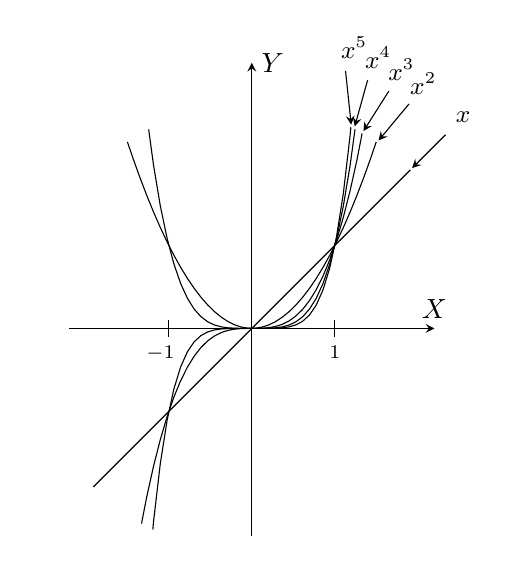
\begin{tikzpicture}[x=3em,y=3em]
\draw[-stealth] (0,-2.5) -- (0,3.2) node[right] {$Y$}; 
\draw[-stealth] (-2.2,0) -- (2.2,0) node[above] {$X$};
\draw[stealth-] (45:2.73)--(45:3.3);
\draw[stealth-] (56:2.73)--(55:3.3);
\draw[stealth-] (60.5:2.73)--(60:3.3);
\draw[stealth-] (63:2.73)--(65:3.3);
\draw[stealth-] (64:2.73)--(70:3.3);
%
\draw (45:3.6) node {\small $x$};
\draw (55:3.6) node {\small $x^2$};
\draw (60:3.6) node {\small $x^3$};
\draw (65:3.6) node {\small $x^4$};
\draw (70:3.6) node {\small $x^5$};
\draw (1,.1)--(1,-.1) node[below] {\scriptsize $1$};
\draw (-1,.1)--(-1,-.1);
\draw (-1.1,-.1) node[below] {\scriptsize $-1$};
%
\clip (0,0) circle (2.7);
\draw (-2.7,-2.7) --(2.7,2.7);
\draw[domain=-2:2,samples=50,variable=\x] plot (\x,{pow(\x,2)});
\draw[domain=-2:2,samples=50,variable=\x] plot (\x,{pow(\x,3)});
\draw[domain=-2:2,samples=50,variable=\x] plot (\x,{pow(\x,4)});
\draw[domain=-2:2,samples=50,variable=\x] plot (\x,{pow(\x,5)});
%\draw[thick,domain=-7:7,samples=50,variable=\x] plot (\x,{cos(\x r)});
\end{tikzpicture}
\end{center}

\begin{center}
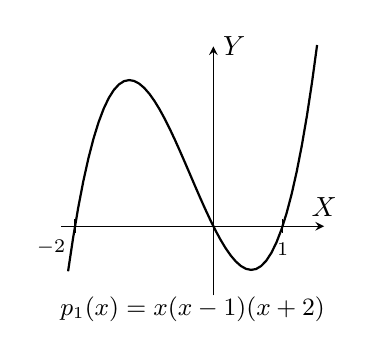
\begin{tikzpicture}[x=2.5em,y=2.5em]
\draw[-stealth] (0,-1) -- (0,2.6) node[right] {$Y$}; 
\draw[-stealth] (-2.2,0) -- (1.6,0) node[above] {$X$};
%
\draw[thick,domain=-2.1:1.5,samples=50,variable=\x] plot (\x,{pow(\x,3)+pow(\x,2)-2*\x});
\draw (1,.1)--(1,-.1) node[below] {\scriptsize $1$};
\draw (-2,.1)--(-2,-.1);
\draw (-2,-.3) node[left] {\scriptsize $-2$};
\draw (-.3,-1.2) node {\small $p_1(x)=x(x-1)(x+2)$};
%\draw[thick,domain=-7:7,samples=50,variable=\x] plot (\x,{cos(\x r)});
\end{tikzpicture}
%
\hspace{2em}
%
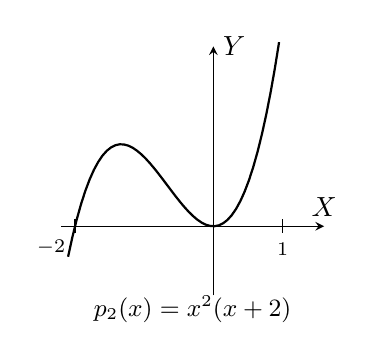
\begin{tikzpicture}[x=2.5em,y=2.5em]
\draw[-stealth] (0,-1) -- (0,2.6) node[right] {$Y$}; 
\draw[-stealth] (-2.2,0) -- (1.6,0) node[above] {$X$};
%
\draw[thick,domain=-2.1:.95,samples=50,variable=\x] plot (\x,{pow(\x,3)+2*pow(\x,2)});
\draw (1,.1)--(1,-.1) node[below] {\scriptsize $1$};
\draw (-2,.1)--(-2,-.1);
\draw (-2,-.3) node[left] {\scriptsize $-2$};
\draw (-.3,-1.2) node {\small $p_2(x)=x^2(x+2)$};
%\draw[thick,domain=-7:7,samples=50,variable=\x] plot (\x,{cos(\x r)});
\end{tikzpicture}\end{center}

%\begin{center}
%\includegraphics{T3/figs/polinomios.pdf}
%\end{center}


\begin{center}
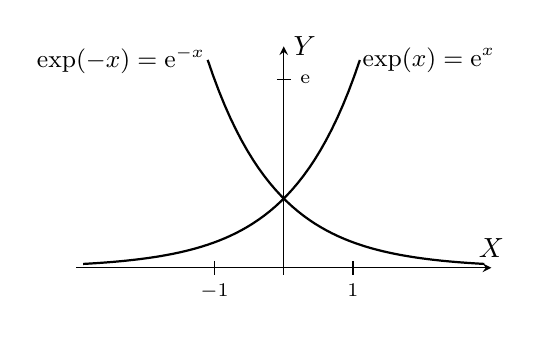
\begin{tikzpicture}[x=2.5em,y=2.5em]
\draw[-stealth] (0,-.1) -- (0,3.2) node[right] {$Y$}; 
\draw[-stealth] (-3,0) -- (3,0) node[above] {$X$};
%
\draw[thick,domain=-2.9:1.1,samples=50,variable=\x] plot (\x,{exp(\x)});
\draw[thick,domain=-1.1:2.9,samples=50,variable=\x] plot (\x,{exp(-\x)});
\draw (1,.1)--(1,-.1) node[below] {\scriptsize $1$};
\draw (-1,.1)--(-1,-.1) node[below] {\scriptsize $-1$};
\draw (-.1,e)--(.1,e) node[right] {\scriptsize $\mathrm e$};
\draw (1,3) node[right] {\small $\exp(x)=\mathrm{e}^x$};
\draw (-1,3) node[left] {\small $\exp(-x)=\mathrm{e}^{-x}$};
%\draw[thick,domain=-7:7,samples=50,variable=\x] plot (\x,{cos(\x r)});
\end{tikzpicture}
%
\hspace{2em}
%
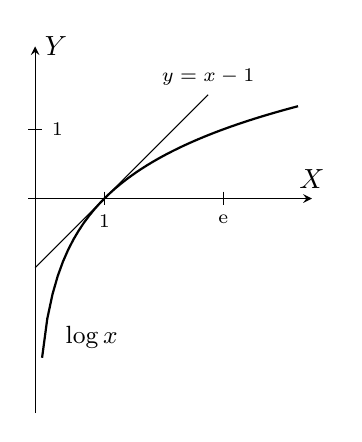
\begin{tikzpicture}[x=2.5em,y=2.5em]
\draw[-stealth] (0,-3.1) -- (0,2.2) node[right] {$Y$}; 
\draw[-stealth] (-.1,0) -- (4,0) node[above] {$X$};
%
\draw[thick,domain=.1:3.8,samples=50,variable=\x] plot (\x,{ln(\x)});
\draw (1,.1)--(1,-.1) node[below] {\scriptsize $1$};
\draw (e,.1)--(e,-.1) node[below] {\scriptsize $\mathrm e$};
\draw (-.1,1)--(.1,1) node[right] {\scriptsize $1$};
\draw (0,-1) -- (2.5,1.5) node[above] {\scriptsize $y=x-1$};
\draw (.3,-2) node[right] {\small $\log x$};
%\draw[thick,domain=-7:7,samples=50,variable=\x] plot (\x,{cos(\x r)});
\end{tikzpicture}
\end{center}

%\begin{center}
%\includegraphics{T3/figs/exp_log.pdf}
%\end{center}


\begin{center}
\begin{minipage}{.6\textwidth}
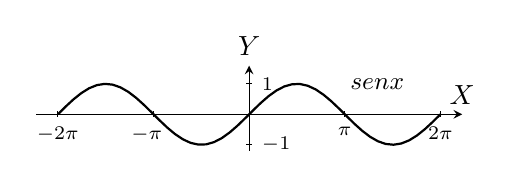
\begin{tikzpicture}[x=1.1em,y=1.1em]
\draw[-stealth] (0,-1.2) -- (0,1.6) node[above] {$Y$}; 
\draw[-stealth] (-7,0) -- (7,0) node[above] {$X$};
%
\draw[thick,domain=-2*pi:2*pi,samples=50,variable=\x] plot (\x,{sin(\x r)});
\draw (pi,.1)--(pi,-.1) node[below] {\scriptsize $\pi$};
\draw (-pi,.1)--(-pi,-.1) node[below] {\scriptsize $-\pi\rule{.6em}{0pt}$};
\draw (2*pi,.1)--(2*pi,-.1) node[below] {\scriptsize $2\pi$};
\draw (-2*pi,.1)--(-2*pi,-.1) node[below] {\scriptsize $-2\pi$};
\draw (-.1,1)--(.1,1) node[right] {\scriptsize $1$};
\draw (-.1,-1)--(.1,-1) node[right] {\scriptsize $-1$};
\draw (3,1) node[right] {\small $\operatorname{sen} x$};
%\draw (-1,3) node[left] {$\exp(-x)=\mathrm{e}^{-x}$};
%
\end{tikzpicture}\\[3em]
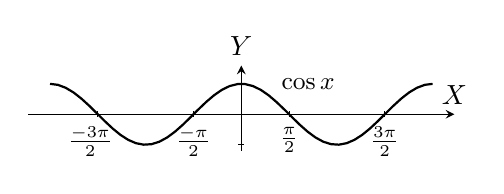
\begin{tikzpicture}[x=1.1em,y=1.1em]
\draw[-stealth] (0,-1.2) -- (0,1.6) node[above] {$Y$}; 
\draw[-stealth] (-7,0) -- (7,0) node[above] {$X$};
%
\draw[thick,domain=-2*pi:2*pi,samples=50,variable=\x] plot (\x,{cos(\x r)});
\draw (.5*pi,.1)--(.5*pi,-.1) node[below] {\small $\frac{\pi}2$};
\draw (1.5*pi,.1)--(1.5*pi,-.1) node[below] {\small $\frac{3\pi}2$};
\draw (-.5*pi,.1)--(-.5*pi,-.1) node[below] {\small $\frac{-\pi}2$};
\draw (-1.5*pi,.1)--(-1.5*pi,-.1) node[below] {\small $\frac{-3\pi}2\rule{.6em}{0pt}$};
%\draw (-.1,1)--(.1,1) node[right] {\small $1$};
\draw (-.1,-1)--(.1,-1);
\draw (1,1) node[right] {\small $\cos x$};
%\draw (-1,3) node[left] {$\exp(-x)=\mathrm{e}^{-x}$};
%
\end{tikzpicture}
\end{minipage}
%
\hspace{-3em}
%
\raisebox{-5em}{
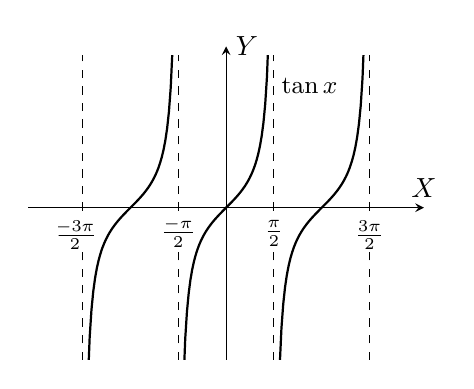
\begin{tikzpicture}[x=1.1em,y=1.1em]
\draw[-stealth] (0,-5) -- (0,5.3) node[right] {$Y$}; 
\draw[-stealth] (-6.5,0) -- (6.5,0) node[above] {$X$};
%
\clip (-5.5,-5) rectangle (5.5,5);
\draw[thick,domain=-4.6:-1.7,samples=50,variable=\x] plot (\x,{tan(\x r)});
\draw[thick,domain=-1.4:1.4,samples=50,variable=\x] plot (\x,{tan(\x r)});
\draw[thick,domain=1.7:4.6,samples=50,variable=\x] plot (\x,{tan(\x r)});
\draw[dashed] (.5*pi,-5)--(.5*pi,-1.4);
\draw[dashed] (.5*pi,-.1)--(.5*pi,5);
\draw[dashed] (1.5*pi,-5)--(1.5*pi,-1.4);
\draw[dashed] (1.5*pi,-.1)--(1.5*pi,5);
\draw[dashed] (-.5*pi,-5)--(-.5*pi,-1.4);
\draw[dashed] (-.5*pi,-.1)--(-.5*pi,5);
\draw[dashed] (-1.5*pi,-5)--(-1.5*pi,-1.4);
\draw[dashed] (-1.5*pi,-.1)--(-1.5*pi,5);
%
\draw (.5*pi,-.1) node[below] {\small $\frac{\pi}2$};
\draw (1.5*pi,-.1) node[below] {\small $\frac{3\pi}2$};
\draw (-.5*pi,-.02) node[below] {\small $\frac{-\pi}2$};
\draw (-1.5*pi,-.1) node[below] {\small $\frac{-3\pi}2\rule{.6em}{0pt}$};
%\draw (-.1,1)--(.1,1) node[right] {\small $1$};
%\draw (.1,-1)--(-.1,-1) node[left] {\small $-1$};
\draw (1.5,4) node[right] {\small $\tan x$};
%\draw (-1,3) node[left] {$\exp(-x)=\mathrm{e}^{-x}$};
%
\end{tikzpicture}
}
\end{center}

\begin{center}
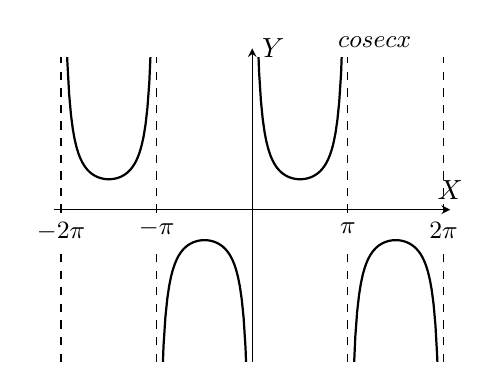
\begin{tikzpicture}[x=1.1em,y=1.1em]
\draw[-stealth] (0,-5) -- (0,5.3) node[right] {$Y$}; 
\draw[-stealth] (-6.5,0) -- (6.5,0) node[above] {$X$};
\draw (2.5,5.5) node[right] {\small $\operatorname{cosec} x$};
\draw (pi,-.1) node[below] {\small $\pi$};
\draw (2*pi,-.1) node[below] {\small $2\pi$};
\draw (-pi,-.02) node[below] {\small $-\pi$};
\draw (-2*pi,-.1) node[below] {\small $-2\pi$};
%\draw (-.1,1)--(.1,1) node[right] {\small $1$};
%\draw (.1,-1)--(-.1,-1) node[left] {\small $-1$};
%\draw (-1,3) node[left] {$\exp(-x)=\mathrm{e}^{-x}$};
%
\clip (-6.5,-5) rectangle (6.5,5);
\draw[thick,domain=-6.2:-3.2,samples=50,variable=\x] plot (\x,{cosec(\x r)});
\draw[thick,domain=-3.1:-.1,samples=50,variable=\x] plot (\x,{cosec(\x r)});
\draw[thick,domain=0.1:3.1,samples=50,variable=\x] plot (\x,{cosec(\x r)});
\draw[thick,domain=3.2:6.2,samples=50,variable=\x] plot (\x,{cosec(\x r)});
\draw[dashed] (pi,-5)--(pi,-1.4);
\draw[dashed] (pi,-.1)--(pi,5);
\draw[dashed] (2*pi,-5)--(2*pi,-1.4);
\draw[dashed] (2*pi,-.1)--(2*pi,5);
\draw[dashed] (-pi,-5)--(-pi,-1.4);
\draw[dashed] (-pi,-.1)--(-pi,5);
\draw[dashed] (-2*pi,-5)--(-2*pi,-1.4);
\draw[dashed] (-2*pi,-.1)--(-2*pi,5);
%
\end{tikzpicture}
\hspace{3em}
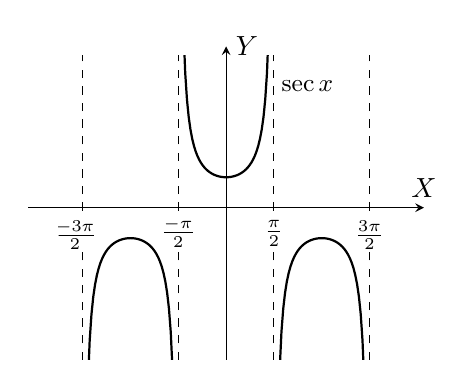
\begin{tikzpicture}[x=1.1em,y=1.1em]
\draw[-stealth] (0,-5) -- (0,5.3) node[right] {$Y$}; 
\draw[-stealth] (-6.5,0) -- (6.5,0) node[above] {$X$};
%
\clip (-5.5,-5) rectangle (5.5,5);
\draw[thick,domain=-4.6:-1.7,samples=50,variable=\x] plot (\x,{sec(\x r)});
\draw[thick,domain=-1.4:1.4,samples=50,variable=\x] plot (\x,{sec(\x r)});
\draw[thick,domain=1.7:4.6,samples=50,variable=\x] plot (\x,{sec(\x r)});
\draw[dashed] (.5*pi,-5)--(.5*pi,-1.4);
\draw[dashed] (.5*pi,-.1)--(.5*pi,5);
\draw[dashed] (1.5*pi,-5)--(1.5*pi,-1.4);
\draw[dashed] (1.5*pi,-.1)--(1.5*pi,5);
\draw[dashed] (-.5*pi,-5)--(-.5*pi,-1.4);
\draw[dashed] (-.5*pi,-.1)--(-.5*pi,5);
\draw[dashed] (-1.5*pi,-5)--(-1.5*pi,-1.4);
\draw[dashed] (-1.5*pi,-.1)--(-1.5*pi,5);
%
\draw (.5*pi,-.1) node[below] {\small $\frac{\pi}2$};
\draw (1.5*pi,-.1) node[below] {\small $\frac{3\pi}2$};
\draw (-.5*pi,-.02) node[below] {\small $\frac{-\pi}2$};
\draw (-1.5*pi,-.1) node[below] {\small $\frac{-3\pi}2\rule{.6em}{0pt}$};
%\draw (-.1,1)--(.1,1) node[right] {\small $1$};
%\draw (.1,-1)--(-.1,-1) node[left] {\small $-1$};
\draw (1.5,4) node[right] {\small $\sec x$};
%\draw (-1,3) node[left] {$\exp(-x)=\mathrm{e}^{-x}$};
%
\end{tikzpicture}

\end{center}

%
%\begin{center}
%\includegraphics{T3/figs/trig-1.pdf}\\
%%\end{center}
%\begin{center}
%\includegraphics{T3/figs/trig-2.pdf}
%\end{center}


\begin{center}
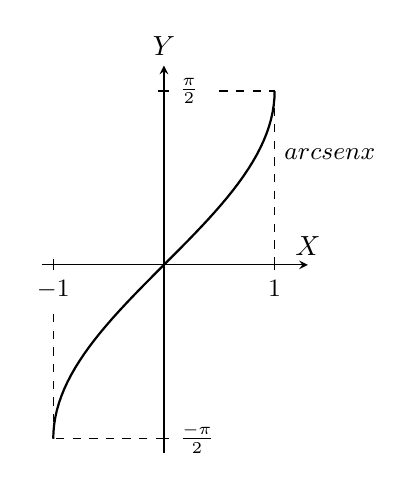
\begin{tikzpicture}[x=4em,y=4em]
\draw[-stealth] (0,-1.7) -- (0,1.8) node[above] {$Y$}; 
\draw[-stealth] (-1.1,0) -- (1.3,0) node[above] {$X$};
\draw (1,1) node[right] {\small $\operatorname{arcsen} x$};
\draw (-.05,.5*pi)--(.05,.5*pi) node[right] {\small $\frac{\pi}2$};
\draw (-.05,-.5*pi)--(.05,-.5*pi) node[right] {\small $\frac{-\pi}2$};
\draw[dashed] (.5,.5*pi)--(1,.5*pi);
\draw[dashed] (0,-.5*pi)--(-1,-.5*pi);
\draw (1,.05)--(1,-.05) node[below] {\small $1$};
\draw (-1,.05)--(-1,-.05) node[below] {\small $-1$};
\draw[dashed] (1,.5*pi)--(1,0);
\draw[dashed] (-1,-.5*pi)--(-1,-.4);
%
\draw[thick,domain=-.5*pi:.5*pi,samples=50,variable=\x] plot ({sin(\x r)},\x);
%
\end{tikzpicture}
\hspace{3em}
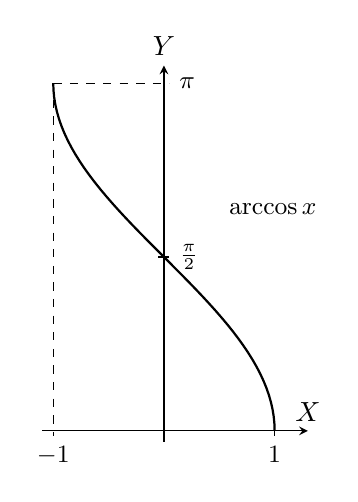
\begin{tikzpicture}[x=4em,y=4em]
\draw[-stealth] (0,-.1) -- (0,3.3) node[above] {$Y$}; 
\draw[-stealth] (-1.1,0) -- (1.3,0) node[above] {$X$};
\draw (.5,2) node[right] {\small $\arccos x$};
\draw[dashed] (-1,pi)--(.05,pi) node[right] {\small $\pi$};
\draw (-.05,.5*pi)--(.05,.5*pi) node[right] {\small $\frac{\pi}2$};
\draw (1,.05)--(1,-.05) node[below] {\small $1$};
\draw[dashed] (-1,pi)--(-1,-.05) node[below] {\small $-1$};
%
\draw[thick,domain=0:pi,samples=50,variable=\x] plot ({cos(\x r)},\x);
%
\end{tikzpicture}

\end{center}

%
%\begin{center}
%\includegraphics{T3/figs/trig_inv1.pdf}
%\end{center}

\begin{center}
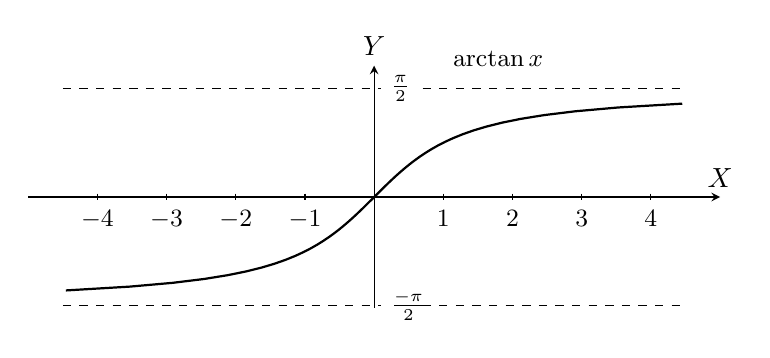
\begin{tikzpicture}[x=2.5em,y=2.5em]
\draw[-stealth] (0,-1.6) -- (0,1.9) node[above] {$Y$}; 
\draw[-stealth] (-5,0) -- (5,0) node[above] {$X$};
\draw (1,2) node[right] {\small $\arctan x$};
\draw[dashed] (-4.5,.5*pi)--(.1,.5*pi) node[right] {\small $\frac{\pi}2$};
\draw[dashed] (.7,.5*pi)--(4.5,.5*pi);% node[right] {\small $\pi$};
\draw[dashed] (-4.5,-.5*pi)--(.1,-.5*pi) node[right] {\small $\frac{-\pi}2$};
\draw[dashed] (.7,-.5*pi)--(4.5,-.5*pi);% node[right] {\small $\pi$};
\draw (1,.05)--(1,-.05) node[below] {\small $1$};
\draw (2,.05)--(2,-.05) node[below] {\small $2$};
\draw (3,.05)--(3,-.05) node[below] {\small $3$};
\draw (4,.05)--(4,-.05) node[below] {\small $4$};
\draw (-1,.05)--(-1,-.05) node[below] {\small $-1$};
\draw (-2,.05)--(-2,-.05) node[below] {\small $-2$};
\draw (-3,.05)--(-3,-.05) node[below] {\small $-3$};
\draw (-4,.05)--(-4,-.05) node[below] {\small $-4$};
%\draw[dashed] (-1,pi)--(-1,-.05) node[below] {\small $-1$};
%
\draw[thick,domain=-1.35:1.35,samples=50,variable=\x] plot ({tan(\x r)},\x);
%
\end{tikzpicture}
\end{center}
%
%\begin{center}
%\includegraphics{T3/figs/trig_inv2.pdf}
%\end{center}
%
\begin{center}
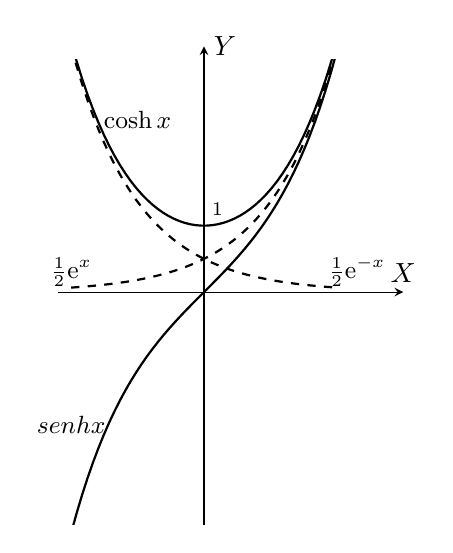
\begin{tikzpicture}[x=2.4em,y=2.4em]
\draw[-stealth] (0,-3.5) -- (0,3.7) node[right] {$Y$}; 
\draw[-stealth] (-2.2,0) -- (3,0) node[above] {$X$};
%
\draw (-1,2.6) node {\small $\cosh x$};
\draw (-2,.3) node {\small $\frac12\mathrm{e}^x$};
\draw (2.3,.3) node {\small $\frac12\mathrm{e}^{-x}$};
\draw (-2,-2) node {\small $\operatorname{senh} x$};
\draw (.2,1) node[above] {\scriptsize $1$};
%
\clip  (-2,-3.5) rectangle (2,3.5);
\draw[thick,domain=-2:2,samples=50,variable=\x] plot (\x,{.5*exp(\x)+.5*exp(-\x)});
\draw[thick,dashed,domain=-2:2,samples=50,variable=\x] plot (\x,{.5*exp(\x)});
\draw[thick,dashed,domain=-2:2,samples=50,variable=\x] plot (\x,{.5*exp(-\x)});
\draw[thick,domain=-2:2,samples=50,variable=\x] plot (\x,{.5*exp(\x)-.5*exp(-\x)});
\end{tikzpicture}
\end{center}

%\begin{center}
%\includegraphics{T3/figs/hiperbolicas.pdf}
%\end{center}
%
%\begin{center}
%\includegraphics{T3/figs/hiperb_inv.pdf}
%\end{center}

%\begin{center}
%\includegraphics{T3/figs/potenciales.pdf}
%\end{center}

\begin{center}
\begin{tikzpicture}[x=3.5em,y=3.5em]
\draw[-stealth] (0,-2.1) -- (0,2.2) node[right] {$Y$}; 
\draw[-stealth] (-1.6,0) -- (1.6,0) node[above] {$X$};
%
\draw (0,2.3) node[above] {\small $f(x)=\dfrac{1}{4(2x-1)(2x+1)}$};
%
\clip  (-1.5,-2) rectangle (1.5,2);
\draw[thick,domain=-1.5:-.51,samples=50,variable=\x] plot (\x,{divide(1,16*\x*\x-4)});
\draw[thick,domain=-.49:.49,samples=50,variable=\x] plot (\x,{divide(1,16*\x*\x-4)});
\draw[thick,domain=.51:1.5,samples=50,variable=\x] plot (\x,{divide(1,16*\x*\x-4)});
\draw[dashed] (-.5,2)--(-.5,-.05) node[below] {$\frac{-1}2$};
\draw[dashed] (-.5,-.6) -- (-.5,-2) ;
\draw[dashed] (.5,2)--(.5,-.05) node[below] {$\frac12$};
\draw[dashed] (.5,-.6) -- (.5,-2) ;
\end{tikzpicture}
\hspace{3em}
\begin{tikzpicture}[x=3.5em,y=3.5em]
\draw[-stealth] (0,-2.1) -- (0,2.2) node[right] {$Y$}; 
\draw[-stealth] (-1.6,0) -- (1.6,0) node[above] {$X$};
%
\draw (0,2.3) node[above] {\small $f(x)=\dfrac{7x^2}{4(2x-1)(2x+1)}$};
%
\clip  (-1.5,-2) rectangle (1.5,2);
\draw[thick,domain=-1.5:-.51,samples=50,variable=\x] plot (\x,{divide(7*\x*\x,16*\x*\x-4)});
\draw[thick,domain=-.49:.49,samples=50,variable=\x] plot (\x,{divide(7*\x*\x,16*\x*\x-4)});
\draw[thick,domain=.51:1.5,samples=50,variable=\x] plot (\x,{divide(7*\x*\x,16*\x*\x-4)});
\draw[dashed] (-.5,2)--(-.5,-.05) node[below] {$\frac{-1}2$};
\draw[dashed] (-.5,-.6) -- (-.5,-2) ;
\draw[dashed] (.5,2)--(.5,-.05) node[below] {$\frac12$};
\draw[dashed] (.5,-.6) -- (.5,-2) ;
\draw[dashed] (-1.5,.4375)--(.01,.4375) node[right] {$\frac7{16}$};
\draw[dashed] (.5,.4375) -- (1.5,.4375) ;
\end{tikzpicture}
\end{center}
\enlargethispage{2cm}


\begin{center}
\begin{tikzpicture}[x=3.5em,y=3.5em]
\draw[-stealth] (0,-2.1) -- (0,2.2) node[right] {$Y$}; 
\draw[-stealth] (-1.6,0) -- (1.6,0) node[above] {$X$};
%
\draw (0,2.3) node[above] {\small $f(x)=\dfrac{7x^3}{4(2x-1)(2x+1)}$};
%
\clip  (-1.5,-2) rectangle (1.5,2);
\draw[thick,domain=-1.5:-.51,samples=50,variable=\x] plot (\x,{divide(7*\x*\x*\x,16*\x*\x-4)});
\draw[thick,domain=-.49:.49,samples=50,variable=\x] plot (\x,{divide(7*\x*\x*\x,16*\x*\x-4)});
\draw[thick,domain=.51:1.5,samples=50,variable=\x] plot (\x,{divide(7*\x*\x*\x,16*\x*\x-4)});
\draw[dashed] (-.5,2)--(-.5,-.05) node[below] {$\frac{-1}2$};
\draw[dashed] (-.5,-.6) -- (-.5,-2) ;
\draw[dashed] (.5,2)--(.5,-.05) node[below] {$\frac12$};
\draw[dashed] (.5,-.6) -- (.5,-2) ;
\draw[dashed] (-1.5,-.65625) -- (-.75,-.328125);
\draw[dashed] (-.25,-.109375) -- (1.5,.65625);
\end{tikzpicture}
\hspace{3em}
\begin{tikzpicture}[x=3.5em,y=3.5em]
\draw[-stealth] (0,-2.1) -- (0,2.2) node[right] {$Y$}; 
\draw[-stealth] (-1.6,0) -- (1.6,0) node[above] {$X$};
%
\draw (0,2.3) node[above] {\small $f(x)=\dfrac{7x^4}{4(2x-1)(2x+1)}$};
%
\clip  (-1.5,-2) rectangle (1.5,2);
\draw[thick,domain=-1.5:-.51,samples=50,variable=\x] plot (\x,{divide(7*\x*\x*\x*\x,16*\x*\x-4)});
\draw[thick,domain=-.49:.49,samples=50,variable=\x] plot (\x,{divide(7*\x*\x*\x*\x,16*\x*\x-4)});
\draw[thick,domain=.51:1.5,samples=50,variable=\x] plot (\x,{divide(7*\x*\x*\x*\x,16*\x*\x-4)});
\draw[dashed] (-.5,2)--(-.5,-.05);
\draw (-.6,-.05) node[below] {$\frac{-1}2$};
\draw[dashed] (-.5,-.6) -- (-.5,-2) ;
\draw[dashed] (.5,2)--(.5,-.05);
\draw (.6,-.05) node[below] {$\frac12$};
\draw[dashed] (.5,-.6) -- (.5,-2) ;
\end{tikzpicture}
\end{center}

%
%\begin{center}
%\includegraphics{T3/figs/racionales.pdf}
%\end{center}
%

\newpage



\section{Ecuaciones y sistemas de ecuaciones}\label{lec:ec-sist}

La resolución de ecuaciones y sistemas de ecuaciones es una herramienta básica en el desarrollo de múltiples ejercicios tanto de matemáticas como de otras materias científicas.
Las técnicas de resolución se basan en las propiedades básicas de las operaciones algebraicas. 
Aunque el alumno debe conocer las técnicas básicas para el estudio de ecuaciones, en los ejemplos que componen esta sección establecemos algunas pautas, indicaciones y advertencias.

\begin{ejemplo}
Vamos a resolver la ecuación
\[
\sqrt{x}= \sqrt{x^2+x-1},\qquad x\in \mathbb{R}.
\]
Antes de empezar, recordemos que, cuando trabajamos con números reales, $\sqrt{x}$ representa la raíz positiva; 
de esta forma, si queremos expresar la raíz negativa, escribiremos $-\sqrt{x}$.

El primer paso en la resolución es elevar al cuadrado ambos lados de la igualdad para eliminar las raíces, pero además tendremos que descartar las soluciones que lleven a radicandos negativos, es decir, la ecuación es equivalente a:
\[
x= x^2+x-1,\quad x\ge 0,
% \qquad\quad
%-x= x^2+x-1,
\]
De la misma forma, la raíz cuadrada ``cancela'' un cuadrado, pero el resultado debe ser positivo, por lo que el resultado debe escribirse con valor absoluto:
\[
\sqrt{a^2} = \sqrt{|a|^2}=|a|, \text{ para todo } a\in\mathbb{R}.
\]
Siguiendo con la ecuación del ejemplo:
\[
x= x^2+x-1,\ x\ge0 \quad\Rightarrow\quad 0= x^2-1,\ x\ge 0\quad\Rightarrow\quad x=1.
\]
Obsérvese que, en el último paso, hemos descartado la raíz negativa de~1.\fej
\end{ejemplo}
%
\begin{ejemplo}
Vamos a resolver la ecuación
\[
x^3- 2x^2+x=0.
\]
Un error bastante frecuente es efectuar directamente la siguiente simplificación:
\[
x^2-2x+1=0.
\]
Hacemos esto porque dividimos ambos lados entre $x$, pero para hacer esto, debemos suponer que $x\ne0$.
Es preferible razonar de la siguiente forma:
sacando factor común $x$ en la ecuación, obtenemos
\[
x(x^2-2x+1)=0,
\]
Dado que el producto de dos números es cero si y solo si uno de los dos lo es, esta ecuación se convierte en dos ecuaciones que debemos estudiar por separado:
\[
x=0,\qquad\quad x^2-2x+1=0
\]
La primera es trivial y la segunda lleva a la solución $x=1$.

La factorización de expresiones es, en general, una técnica bastante útil para la resolución de ecuaciones, como iremos comprobando en el curso.\fej
\end{ejemplo}
%
\begin{ejemplo}
De los sistemas de ecuaciones, solo los denominados \emph{sistemas lineales} son resolubles de manera mecánica; es decir, siempre es posible decidir si tienen o no soluciones y, en tal caso, determinarlas.
Entendemos que el alumno debe conocer la teoría básica asociada a estos sistemas, así que solo vamos a resolver un ejemplo para insistir en que el método más simple y eficiente para resolverlos es el denominado \emph{método de Gauss} o \emph{reducción}.


En el desarrollo siguiente, utilizamos etiquetas para indicar para las operaciones realizadas:
$(e2)-(e1)\rightarrow(e2)$ indica que restamos la primera a la segunda ecuación y que el resultado pasa a ser la nueva segunda ecuación.
%; $2\ast(e2)$ indica que la segunda ecuación se multiplica por 2 y
% que el resultado pasa a ser la nueva segunda ecuación.
%
\begin{multline*}
\left\{\begin{array}{rl}
x+y-z & =1\\
x+2y+2z &=2 \\
-x+y+3z &= -2
\end{array}\right\}
\overset{(e2)-(e1)\rightarrow(e2)}{\Longrightarrow}
\left\{\begin{array}{rl}
x+y-z & =1\\
 y+3z &=1 \\
-x+y+3z &= -2
\end{array}\right\} \\
\overset{(e3)+(e1)\rightarrow(e3)}{\Longrightarrow}\left\{\begin{array}{rl}
x+y-z & =1\\
 y+3z &=1 \\
2y+2z &= -1
\end{array}\right\}
\overset{(e3)-2*(e2)\rightarrow (e3) }{\Longrightarrow}
%\left\{\begin{array}{rl}
%x+y-z & =1\\
%2y+6z &=2 \\
%2y+2z &= -1
%\end{array}\right\} \\
%\overset{(e3)-(e2)}{\Rightarrow}
\left\{\begin{array}{rl}
x+y-z & =1\\
2y+6z &=2 \\
-4z &= -3
\end{array}\right\}
\end{multline*}
El objetivo ha sido obtener un sistema ``triangular'', que se resuelve fácilmente de abajo hacia arriba.
\[
\rule{0pt}{0pt}\hspace{-1.3em}
\left.\begin{array}{r}
\left.\begin{array}{r}
(e3)\Rightarrow \fbox{$z=\dfrac34$}\\
(e2)
\end{array}\right\}\Rightarrow 2y+6\dfrac34 =2 \Rightarrow \fbox{$y=-\dfrac54$}\\
(e1)
\end{array}
\right\}
\Rightarrow x-\frac54-\frac34 =1 \Rightarrow \fbox{$x=3$}
\fejeq
\]
\end{ejemplo}

%\begin{tcolorbox}[breakable,title=\subsection{Sistemas de ecuaciones no lineales}]
%...
%\end{tcolorbox}


\subsection{Sistemas de ecuaciones no lineales}

Para los sistemas no lineales, no disponemos de algoritmos similares al de Gauss para calcular, si existe, la solución de cualquier sistema.
En estos casos, solo podemos utilizar ``heurísticas'', es decir, reglas que, sin ser generales, son aplicables a muchos casos y, por lo tanto, es recomendable utilizarlas en primer lugar.
No obstante, solo la experiencia y la intuición ayudarán a abordar con éxito este tipo de problemas.
%
\begin{enumerate}
\item
\emph{Sustitución:}
Buscamos una ecuación que permita despejar fácilmente una variable, directamente o a partir de una factorización que divida el sistema en varios casos.
La variable despejada se sustituye en el resto de las ecuaciones, obteniendo uno o varios sistemas con menos variables.
\item
\emph{Igualación:}
Si una de las variables se puede despejar en todas las ecuaciones en las que aparece, podemos hacerlo y a partir de ahí, generar por igualación un sistema equivalente pero con menos variables.

\item
\emph{Reducción:}
Este método de simplificación consiste en sumar o restar ecuaciones, posiblemente multiplicadas por constantes o por expresiones; el proceso es similar al utilizado en sistemas lineales.
Aunque no consigamos eliminar una variable, intentaremos reducir de esta forma la complejidad de las ecuaciones antes de aplicar las otras técnicas.
\end{enumerate}

En los ejemplos siguientes mostramos cómo aplicar las técnicas anteriores.

\begin{ejemplo}
Para resolver el sistema
\[
\left\{\begin{array}{rc}
x^2-y=5& \\
3x-y=1&
\end{array}\right.
\]
nos fijamos en la segunda ecuación, que permite despejar fácilmente una variable en función de la otra.
\[
\left.\begin{array}{r}
(e2) \Rightarrow\ y=3x-1\\
(e1)\ x^2-y=5
\end{array}\right\}\quad \Rightarrow\quad x^2-3x+1=5\quad \Rightarrow\quad x=4,\ x=-1
\]
Debemos tener cuidado al escribir las soluciones de un sistema y asociar correctamente los distintos valores que tome cada variable.
En este ejemplo, $x=4$ conduce a $y=11$, mientras que $x=-1$ conduce a $y=-4$;
por lo tanto, debemos escribir las soluciones dejando claras las asociaciones correctas:
\[
\{x_1=4, y_1=11\},\qquad \{x_2=-1, y_2=-4\}.\fejeq
\]
\end{ejemplo}
%
En los sistemas de ecuaciones lineales caben tres posibilidades: que no tengan solución, que tengan solamente una solución o que tengan infinitas soluciones.
Como podemos ver en el ejemplo anterior, en los sistemas no lineales tenemos más posibilidades y puede haber más de una solución aunque estas no sean infinitas.
%
\begin{ejemplo}
En el sistema
\[
\left\lbrace\begin{array}{l} 2x-xy=0 \\ x-yz=0 \\ x^2+y^2+z^2=1,\qquad
x,y,z\in\mathbb{R},\end{array}\right.
\]
elegimos en primer lugar la primera ecuación para factorizarla, sacando $x$ como factor común:
\[
0=2x-xy=x(2-y).
\]
De esta forma, obtenemos dos posibilidades, o bien $x=0$, o bien $y=2$, lo que permite simplificar las otras ecuaciones para obtener dos sistemas más sencillos:
\[
(1)\left\lbrace\begin{array}{l} x=0 \\ yz=0 \\ y^2+z^2=1 \end{array}\right.
\qquad\qquad
(2)\left\lbrace\begin{array}{l} y=2 \\ x-2z=0 \\ x^2+4+z^2=1 \end{array}\right.
\]
La segunda ecuación de (1), conduce a dos posibilidades, o bien $y=0$, o bien $z=0$, que generan dos sistemas triviales:
\[
(1.{}1)\left\lbrace\begin{array}{l} x=0 \\ y=0 \\ z^2=1 \end{array}\right.
\qquad\qquad
(1.{}2)\left\lbrace\begin{array}{l} x=0 \\ z=0 \\ y^2=1 \end{array}\right.
\]
Las soluciones obtenidas a partir de estos son
\[
\begin{array}{c@{,\qquad}c}
\{x_1=0,y_1=0,z_1=-1\} & 
\{x_2=0,y_2=0,z_2=1\},\\
\{x_3=0,y_3=-1,z_3=0\} &
\{x_4=0,y_4=1,z_4=0\}.
\end{array}
\]
El sistema (2) no tiene soluciones en $\mathbb{R}$, ya que su tercera ecuación es equivalente a
$x^2+z^2=-3$.\fej
%En la siguiente lección introduciremos los \emph{números complejos}, con los que podremos expresar más soluciones para este sistema.
%En el sistema (2), elegimos la segunda ecuación para deducir que $x=2z$; llevando esta sustitución a la tercera ecuación llegamos a $4z^2+z^2+4=0$, por lo que
%$z=\pm2\mathrm{i}/\sqrt5$.
%Las últimas soluciones del sistema son
%\[
%\{x_5=\frac{4\mathrm{i}}{\sqrt5},y_5=2,z_5=\frac{2\mathrm{i}}{\sqrt5}\},\qquad 
%\{x_6=-\frac{4\mathrm{i}}{\sqrt5},y_6=2,z_6=-\frac{2\mathrm{i}}{\sqrt5}\}.\fejeq
%\]
\end{ejemplo}
%
\begin{ejemplo}
Vamos a resolver el sistema
\[
\left\{\begin{array}{cl}
&x^2+y^2=1\\
&x=yz\\
&y=xz+1
\end{array}\right.
\]
La variable $z$ aparece en las ecuaciones segunda y tercera, y en ambas podemos despejarla fácilmente:
\begin{equation}
z=\frac{x}{y}\qquad\qquad
z=\frac{y-1}x\label{ej:igualacion}
\end{equation}
Dado que hemos dividido entre $x$ e $y$, posteriormente tendremos que analizar los casos en que $x=0$ o $y=0$.
Aplicando \emph{igualación} en las ecuaciones anteriores obtenemos
\[
\frac{x}{y}=\frac{y-1}x\quad\Rightarrow\quad x^2-y^2+y=0,
\]
por lo que nuestro sistema inicial se ha convertido en
\begin{align*}
& x^2+y^2-1=0\\
& x^2-y^2+y=0
\end{align*}
Ahora vemos que podemos simplificar fácilmente el término $x^2$ restando las dos ecuaciones, para llegar a una ecuación en $y$:
\[
2y^2-y-1=0\qquad\Rightarrow\qquad y=1,\ y=\frac{-1}2.
\]
Utilizando la primera ecuación, $x^2+y^2-1=0$, y que $z=\dfrac{x}{y}$, completamos la resolución:
\begin{multline*}
\{x_1=0, y_1=1, z_1=0\},\qquad \{x_2=\frac{\sqrt3}2,y_2=\frac{-1}2, z_2=-\sqrt3\},\\
\{x_3=\frac{-\sqrt3}2,y_3=\frac{-1}2, z_3=\sqrt3\}.
\end{multline*}
Finalmente, debemos analizar qué ocurre si $x=0$ o $y=0$.
El caso $x=0$ conduce fácilmente a la primera solución obtenida anteriormente.
Por la segunda ecuación, si $y=0$, entonces $x=0$, lo cual es imposible atendiendo a la primera ecuación del sistema inicial.\fej
\end{ejemplo}

\newpage

%\thispagestyle{empty}
%
%\ 
%
%\vfill
%\begin{center}
%(Esta página se ha dejado intencionalmente en blanco)
%\end{center}
%\newpage
%


\section{El binomio de Newton}

La fórmula del binomio de Newton permite expandir cualquier potencia de una suma de expresiones, es decir, vamos a generalizar la igualdad
\[
(a+b)^2 = a^2 + 2ab + b^2
\]
a cualquier exponente natural.
Para expandir una potencia como $(a+b)^7$, bastaría con multiplicar siete veces la expresión $(a+b)$, eliminando los paréntesis adecuadamente con la propiedad distributiva;
el binomio de Newton es simplemente una fórmula que nos ``ahorra'' parte de ese trabajo.


\subsection{La Fórmula del Binomio de Newton}

En la fórmula del Binomio de Newton vamos a utilizar unos cuantos elementos que debemos introducir previamente: \emph{factorial}, \emph{números combinatorios} y \emph{sumatorios}.
%
\begin{definicion}[Factorial]
Definimos el \emph{factorial} de un número natural $n$, denotado por $n!$, como sigue:
%
\begin{align*}
0! &= 1 \\
n! &= (n-1)!\cdot n\quad \mbox{ para todo } n\ge 1
\end{align*}
%
\end{definicion}
%
Esta forma de definir una función se denomina \emph{recursiva}:
%:ref informatic
la definición llama al mismo operador que se define, pero aplicado a un número menor, hasta llegar a un \emph{caso base}, en este caso $0!$.
Otra forma de escribir la definición del operador es
\[
n! = 1\cdot 2\cdot 3\cdot \ldots \cdot n,\quad\text{para todo } n\ge1
\]
%
\begin{ejemplo-br}
\begin{itemize}
\item[]
$0! = 1,\qquad 1!=1,\qquad 2!=1\cdot 2=2,
\qquad 3!=1\cdot 2\cdot 3 = 6 $ 
\item[] $10!=1\cdot 2\cdot 3\cdot \ldots\cdot 10 = 3\,628\,800$\fej
%\item $25!=15\,511\,210\,043\,330\,985\,984\,000\,000 $
\end{itemize}
\end{ejemplo-br}

\begin{definicion}[Números combinatorios]
Sean $n$ y $k$ dos números naturales tales que $0\le k \le n$. Se define el \emph{número combinatorio} $\displaystyle\binom{n}{k}$, que se lee ``$n$ sobre $k$'', como 
\[%\label{d:comb1}
\binom{n}{k} = \frac{n!}{k!\cdot(n-k)!}
\]
\end{definicion}
%
\begin{ejemplo}\label{ej:comb}\rule{0pt}{0pt}
%contiene a lo que era \label{pr:comb}
\begin{itemize}
\item %\label{binom107}
$\displaystyle\binom{10}{7} =
\dfrac{10!}{7!\cdot 3!} =
\dfrac{10\cdot 9\cdot 8\cdot \cancel{7!}}{\cancel{7!}\cdot 3!} =
\dfrac{10\cdot 9\cdot 8}{3!} =
\dfrac{10\cdot 9\cdot 8}{3\cdot 2} =
10\cdot 3\cdot 4=120$

\item
$\displaystyle\binom{0}{0} = \frac{0!}{0!\cdot 0!} = 1$

%\item
%\binom{5}{2} = \frac{5!}{2!\cdot 3!} = 10,\quad

\item\label{binomn0}
$\displaystyle\binom{n}{0} =\dfrac{n!}{0!\cdot n!} =\dfrac{n!}{n!} =1$\hfill

\item\label{binomnn}
$\displaystyle\binom{n}{n} =\dfrac{n!}{n!\cdot 0!} =\dfrac{n!}{n!} =1$\hfill

\item\label{binomnk}
$\displaystyle\binom{n}{k}=\frac{n!}{k!\cdot(n-k)!}=\binom{n}{n-k}$\fej
\end{itemize}
\end{ejemplo}

La forma habitual de calcular los números combinatorios es la que se ha utilizado en el primer apartado del ejemplo anterior, es decir, se expande parcialmente el factorial del numerador y se simplifica con el denominador.
Esto lo podemos hacer de forma general para obtener una expresión alternativa para los números combinatorios.
%
\begin{multline*}%\label{d:comb2}
\binom{n}{k} = \frac{n!}{k!\cdot(n-k)!}
= \frac{n(n-1)\ldots(n-k+1)\cdot\cancel{(n-k)!}}{k!\cdot\cancel{(n-k)!}}=\\
=\frac{n(n-1)\ldots(n-k+1)}{k!}
\end{multline*}
%
Obsérvese que en el numerador de la expresión obtenida hay exactamente $k$ factores.
%Esta fórmula es aplicable incluso si $n$ es un número real, sea o no mayor que~$k$, lo que permite generalizar la definición de los números combinatorios.
%%
%\begin{definicion}[Números combinatorios]
%Sea $x$ un número real y $k$ un número natural. Se define el \emph{número combinatorio}
%$\displaystyle\binom{x}{k}$, que se lee ``$x$ sobre $k$'', como 
%\[
%\binom{x}{0}=1,\quad \binom{x}{k} = \frac{x(x-1)\ldots(x-k+1)}{k!}\text{ si }k>0
%\]
%\end{definicion}
%%
%Para recordar esta fórmula, es útil tener en cuenta que el número de factores en el numerador debe ser exactamente $k$.
%%
%\begin{ejemplo}
%\[
%\binom{1/3}{4} = \frac{(1/3)\cdot(-2/3)\cdot(-5/3)\cdot(-8/3)}{4!}
%=-\frac{2\cdot5\cdot\cancel8}{3^4\cdot\cancel4\cdot 3\cdot \cancel2}= -\frac{10}{243}
%\fejeq
%\]
%\end{ejemplo}
%
%Igual que para el factorial, es posible definir el operador ``sobre $k$'' de forma recursiva sobre el natural $k$.
%Aunque tal definición no es necesaria para evaluarlo normalmente, es conveniente conocer este tipo de definiciones para poder implementarlas con lenguajes de programación.
%Una posible definición es la siguiente:
%\begin{align*}
%\binom{x}{0} &=1\\
%\binom{x}{k} &= \frac{x-k+1}{k}\binom{x}{k-1},\text{ si }k>0
%\end{align*}

La siguiente propiedad es la más importante de los números combinatorios, siendo el fundamento del \emph{triángulo de Tartaglia-Pascal}, que veremos a continuación, y permite calcular los números combinatorios de forma recursiva.
%, y del \emph{binomio de Newton}.
%%
%%Algunas propiedades de los números combinatorios son las siguientes:
%%si $n$ y $k$ son dos números naturales tales que $0\le k \le n$,
%%se verifican las siguientes propiedades:
%%
\begin{teorema}[de Pascal]\label{pr:comb}
Para todo $n\in\mathbb{N}$ y todo $k\in\mathbb{N}$:
\[
\binom{n}{k}+\binom{n}{k+1}=\binom{n+1}{k+1}
\]
\end{teorema}
%
\begin{ejemplo}
En este ejemplo, mostramos cómo se llega a esta igualdad en un caso particular; por esta razón, evitamos la realización de la mayoría de los cálculos intermedios. Este tipo de desarrollos nos ayudan a entender demostraciones generales, en las que manejamos variables y parámetros en lugar de números concretos.
%
\begin{multline*}
\binom{8}{3}+\binom{8}{4}=
\dfrac{8\cdot 7\cdot 6}{3!}+
\dfrac{8\cdot 7\cdot 6\cdot 5}{4!} =
\dfrac{4\cdot 8\cdot 7\cdot 6}{4\cdot 3!}+
\dfrac{8\cdot 7\cdot 6\cdot 5}{4!} =\\
=\dfrac{4\cdot 8\cdot 7\cdot 6+8\cdot 7\cdot 6\cdot 5}{4!}=
\dfrac{(4+5)\cdot 8\cdot 7\cdot 6}{4!}=
\dfrac{9\cdot 8\cdot 7\cdot 6}{4!}=\binom{9}{4}\fejeq
\end{multline*}
\end{ejemplo}
%
\paragraph{Triángulo de Tartaglia-Pascal.}
El teorema de Pascal permite calcular los números combinatorios usando una representación geométrica que se donomina \emph{triángulo de Tartaglia} o \emph{triángulo de Tartaglia-Pascal}.
Construimos este triángulo colocando en el vértice superior, el número $\binom00$ y debajo de él colocamos los números $\binom10$ y $\binom11$; formamos así un primer triángulo con solo tres números.
A partir de aquí, vamos añadiendo nuevas filas usando la siguiente regla:
debajo de cada par de números, colocamos su suma:
\[
\begin{array}{ccccc}
\binom{n}{k} &&&& \binom{n}{k+1}\\
 & \searrow & & \swarrow & \\
&&\binom{n}{k}+\binom{n}{k+1}&&
\end{array}
\quad
\stackrel{\text{T. Pascal}}{=}
\quad
\begin{array}{ccccc}
\binom{n}{k} &&&& \binom{n}{k+1}\\
 & \searrow & & \swarrow & \\
&&\binom{n+1}{k+1}&&
\end{array}
\]
Adicionalmente, cada fila se comienza con $\binom{n}0=1$ y se termina con $\binom{n}n=1$.
Vemos a continuación el triángulo resultante hasta la quinta fila, a la izquierda con los números combinatorios indicados y a la derecha con los valores resultantes.
\[
\renewcommand{\arraystretch}{1.4}
\begin{array}{c@{\ }c%
@{\ }c%
@{\ }c%
@{\ }c%
@{\ }c%
@{\ }c%
@{\ }c%
@{\ }c%
@{\ }c%
@{\ }c}
& & & & & \binom{0}{0}\\
& & & & \binom{1}{0} & & \binom{1}{1} \\
& & & \binom{2}{0} & & \binom{2}{1} & & \binom{2}{2}\\
& & \binom{3}{0} & & \binom{3}{1} & & \binom{3}{2} & & \binom{3}{3}\\
& \binom{4}{0} & & \binom{4}{1} & & \binom{4}{2} & & \binom{4}{3} & & \binom{4}{4}\\
\binom{5}{0} & & \binom{5}{1} & & \binom{5}{2} & & \binom{5}{3} & & \binom{5}{4} & & \binom{5}{5}
\end{array}
\qquad\quad
\begin{array}{c@{\ }c%
@{\ }c%
@{\ }c%
@{\ }c%
@{\ }c%
@{\ }c%
@{\ }c%
@{\ }c%
@{\ }c%
@{\ }c}
& & & & & 1\\
& & & & 1 & & 1\\
& & & 1 & & 2 & & 1\\
 & & 1 & & 3 & & 3 & & 1\\
& 1 & & 4 & & 6 & & 4 & & 1\\
1 & & 5 & & 10 & & 10 & & 5 & & 1
\end{array}
\]

\paragraph{Operador sumatorio.} El operador $\displaystyle\sum$ o \emph{sumatorio} se utiliza para expresar sumas con un cantidad variable de sumandos:
\[
\sum_{k=m}^n f(k) = f(m)+f(m+1)+\dots+f(n)
\]
Los sumandos se expresan en función de una variable $k$ que tomará valores consecutivos entre dos números naturales $m$ y $n$ tales que $m\le n$.
Por ejemplo,
\[
\sum_{k=2}^5 (2k-1)^2 = 3^2+5^2+7^2+9^2
\]
La variable utilizada como \emph{índice} de cada sumando no influye en el resultado y podremos cambiarla por la letra que deseemos siempre que no interfiera en el resto del problema.
Por ejemplo, en los sumatorios siguientes utilizamos índices distintos pero obtenemos el mismo resultado:
\begin{align*}
& \sum_{k=1}^{10}k=1+2+3+4+5+6+7+8+9+10=55\\
& \sum_{j=1}^{10}j=1+2+3+4+5+6+7+8+9+10=55
\end{align*}
%
El operador sumatorio es frecuente en los lenguajes de programación, en los que toma una sintaxis similar~a
\[
\mathtt{sum}(f(k),k,m,n)
\]

\paragraph{Binomio de Newton.}
Ya tenemos todos los elementos necesarios para expresar la fórmula del binomio de Newton.
%
\begin{teorema}[Fórmula del binomio de Newton]\label{th:newton}
Para todo par de números $a$ y $b$ y todo número natural $n$, se verifica que 
\[
(a+b)^n = \sum_{k=0}^n \binom{n}{k} a^{n-k} b^k
\]
\end{teorema}
%
También podemos escribir la fórmula del binomio usando ``puntos suspensivos'':
\begin{multline*}
(a+b)^n = \sum_{k=0}^n \binom{n}{k} a^{n-k} b^k=\\
= \binom{n}{0}a^n b^0 + \binom{n}{1}a^{n-1} b + \binom{n}{2}a^{n-2} b^2 + \cdots +
\binom{n}{n-1} a b^{n-1} + \binom{n}{n} a^0 b^n.
\end{multline*}
%
\begin{ejemplo-br}
\begin{itemize}
\item $ (x-y)^2 = \binom{2}{0} x^2 (-y)^0 + \binom{2}{1} x (-y) + \binom{2}{2} x^0 (-y)^2
= x^2 - 2xy + y^2 $
\item $ (s+t)^3 = \binom{3}{0} s^3 t^0 + \binom{3}{1} s^2 t + \binom{3}{2} s
t^2 + \binom{3}{3} s^0 t^3 = s^3 + 3s^2t + 3st^2+ t^3 $
\item $ (z-2)^6 = z^6 - 12z^5 + 60z^4 - 160z^3 + 240z^2 - 192z + 64 $
\item
$2^n=(1+1)^n=\binom{n}{0} + \binom{n}{1} + \binom{n}{2}+ \ldots +
\binom{n}{n-1} + \binom{n}{n}$\fej
\end{itemize}
\end{ejemplo-br}

\subsection{Compleción de cuadrados}\label{ss:comp-cuadr}

En la siguiente sección y más adelante a lo largo del curso, vamos a necesitar realizar una transformación sobre polinomios de segundo grado que se denomina \emph{compleción de cuadrados}.
Aunque es una transformación bastante simple, permite resolver muchos problemas: resolución de ecuaciones e inecuaciones de segundo grado, estudio y representación de cónicas, simplificación de expresiones, cálculo de primitivas,\dots

El objetivo de la transformación es que, en la expresión resultante, la variable aparezca solo una vez.
Por ejemplo,
\[
x^2+2x-1 = (x+1)^2-2;
\]
en la expresión de la derecha, la variable $x$ aparece solamente en $(x+1)^2$.
Naturalmente, dado que estamos trabajando con polinomios, en la expresión transformada solo podrán aparecer sumas, restas y productos.
%Transformar mediante \emph{compleción de cuadrados} un polinomio de grado 2, $ax^2+bx+c$ consiste en encontrar los parámetros $A$ y $B$ tales que
%\[
%ax^2+bx+c = a(x+A)^2+B,
%\]
%o bien, encontrar los parámetros $A$, $B$ y $C$ tales que
%\[
%ax^2+bx+c = (Ax+B)^2+C.
%\]
%Hablamos de cuadrados completos porque en las expresiones de la derecha, la variable $x$ aparece solamente un vez y dentro de un cuadrado.
%
\begin{ejemplo}
El primer método para conseguir esta transformación es utilizar identificación de coeficientes.
Por ejemplo, para completar cuadrados en el polinomio $2x^2-3x+1$ podemos buscar parámetros $A$ y $B$ tales que:
\[
2x^2-3x+1 = 2(x+A)^2+B
\]
A partir de aquí, expandiendo la expresión de la derecha e identificando coeficientes, obtenemos un sistema de ecuaciones que permite determinar la expresión buscada.
%
\begin{align*}
2x^2-3x+1 &= 2(x+A)^2+B\\
2x^2-3x+1 &= 2(x^2+2Ax+A^2)+B\\
2x^2-3x+1 &= 2x^2+4Ax+2A^2+B
\end{align*}
Por lo tanto, 
\begin{align*}
&4A=-3\quad \Rightarrow\quad A=\frac{-3}4\\
&2A^2+B = 1\quad \Rightarrow\quad B=1-2\frac9{16}=\frac{-1}8,
\end{align*}
y de ahí: $2x^2-3x+1 = 2\left(x-\dfrac34\right)^2-\dfrac18$.\fej
\end{ejemplo}

Debemos acostumbrarnos, no obstante, a realizar esta transformación de una forma más rápida.
Si nos fijamos en el caso particular $x^2+bx$ y recordamos la fórmula del cuadrado de un binomio, es fácil concluir que la compleción de cuadrados tendrá la siguiente forma:
\[
x^2+bx = \left(x+\frac{b}2\right)^2+\dots
\]
Si elevamos al cuadrado ``mentalmente'', nos aparece el número $b^2/4$, que no está en el lado izquierdo, y por lo tanto debemos ``eliminarlo'', es decir:
\[
x^2+bx = \left(x+\frac{b}2\right)^2-\frac{b^2}4
\]
Si aprendemos a desarrollar mentalmente la igualdad anterior, el proceso de compleción de cuadrados podrá hacerse sin necesidad de recurrir a ecuaciones.
%
\begin{ejemplo}
Vamos a transformar el polinomio $2x^2-4x+1$ usando el proceso explicado anteriormente:
\begin{align*}
2x^2-4x-1 & = 2\left(\underbrace{x^2-2x}-\frac12\right)=\\
& = 2\left(\underbrace{((x-1)^2-1)}-\frac12\right)=\\
& = 2(x-1)^2-2-1=\\
& = 2(x-1)^2-3\tag*{\fej}
\end{align*}
\end{ejemplo}
\begin{rawhtml}
<p></p>
\end{rawhtml}
\begin{ejemplo}
En el ejemplo anterior, hemos sacado factor común al coeficiente de $x^2$ para que los cálculos siguientes sean más simples.
En algunos casos será más sencillo proceder directamente sin hacer este paso. 
%
\begin{align*}
\underbrace{4x^2-3x}+1 & = \Big(\underbrace{\Big(\Big(2x-\frac34\Big)^2-\frac9{16}\Big)}+1\Big)=\\
& = \Big(2x-\frac34\Big)^2+\frac7{16}
\end{align*}
También podemos obtener otras expresiones en las condiciones indicadas:
\begin{align*}
4x^2-3x+1 = \Big(2x-\frac34\Big)^2+\frac7{16}=
\frac{(8x-3)^2}{16}+\frac7{16} = \frac1{16}\Big((8x-3)^2+7\Big)\tag*{\fej}
\end{align*}
\end{ejemplo}
\begin{rawhtml}
<p></p>
\end{rawhtml}
\begin{ejemplo}
Ya hemos resuelto varias ecuaciones de segundo grado aplicando la fórmula que todo estudiante sabe desde sus años de educación primaria.
En realidad, no es más que una consecuencia de la compleción de cuadrados que hemos aprendido en esta sección.
Resolvemos en este ejemplo una ecuación sin utilizar la fórmula y dejamos al alumno el ejercicio de deducir la fórmula para una ecuación general $ax^2+bx+c=0$ siguiendo los mismos pasos.
%
\begin{align*}
x^2-x-2 & = 0 \\
\Big(\Big(x-\frac12\Big)^2-\frac14\Big)-2 & = 0 \\
\Big(x-\frac12\Big)^2-\frac94 & = 0 \\
\Big(x-\frac12\Big)^2 &= \frac94 \\
x-\frac12 = \frac32, \quad &\quad x-\frac12 = -\frac32 \\
x = 2, \quad &\quad x = -1 
\end{align*}
De forma equivalente, también podríamos utilizar compleción de cuadrados y la identidad $A^2-B^2=(A+B)(A-B)$ para factorizar directamente los polinomios.
Por ejemplo, sobre el mismo ejemplo anterior, podemos hacer lo siguiente:
\begin{multline*}
x^2-x-2 = \Big(x-\frac12\Big)^2-\frac94=\Big(x-\frac12\Big)^2-\frac{3^2}{2^2}=\\
=\Big(x-\frac12+\frac32\Big)\Big(x-\frac12-\frac32\Big)
=(x+1)(x-2)
\tag*{\fej}
\end{multline*}

\end{ejemplo}




\newpage

\section{Los números complejos}\label{lec:complejos}

En principio, los \emph{números complejos} que introducimos en esta lección fueron definidos para cubrir una carencia de los números reales: hay ecuaciones polinómicas que no tienen solución en $\mathbb{R}$.
Por ejemplo, no hay ningún número real $x$, tal que $x^2+1=0$.
Aunque esta propiedad los determina, también los utilizaremos para resolver o analizar otros problemas geométricos y trigonométricos.
En el campo de la ingeniería electrónica, los números complejos se usan en la descripción de señales periódicas y en el estudio de redes eléctricas.

\paragraph{Conjuntos numéricos.} 
Antes de introducir los números complejos, es conveniente recordar algunos conceptos.
En concreto, vamos a repasar los conjuntos numéricos y las propiedades que rigen las operaciones dentro de ellos.
En la asignatura de \emph{Estructuras algebraicas para la computación} estudiaremos con detalle la estructura y propiedades de los siguientes conjuntos, aquí nos limitamos a recordar su denominación y notación.

\begin{itemize}
\item
\emph{Números naturales:}\quad $\mathbb{N} =\{ 0,1, 2, 3,\dots\}$.
\item
\emph{Números enteros:}\quad $\mathbb{Z} =\{ 0, 1, 2,  3,\dots\} \cup \{ -1, -2, -3,\dots\}$.
\item
\emph{Números racionales:}\quad $\mathbb{Q}=\left\{ \dfrac{p}{q};\ p, q \text{ enteros primos entre sí}, q\ne 0\right\}$.
\end{itemize}

Finalmente, el conjunto de los \emph{números reales} se denota por $\mathbb{R}$, pero no es posible hacer una descripción constructiva de ellos tal y como hemos hecho con los otros.
Tanto el conjunto de los números racionales como el de los reales con las operaciones de suma y producto, tienen estructura de \emph{cuerpo ordenado}, es decir, en ellos se verifican las propiedades que enunciamos a continuación.

\begin{itemize}
\item
\emph{Asociatividad:}
Todos los números reales $a$, $b$ y $c$ verifican
\[
(a+b)+c=a+(b+c),\qquad (a\cdot b)\cdot c=a\cdot (b\cdot c)
\]
\item
\emph{Existencia de elemento neutro y de unidad:} el número $0$ es el elemento neutro para la suma y el número $1$ es la unidad para el producto, es decir, para todo número real $a$
\[
a+0=0+a=a,\qquad
a\cdot 1=1\cdot a=a
\]
\item
\emph{Existencia de elementos opuestos e inversos:}
el número $-a$ es el opuesto de $a$ respecto de la suma, es decir,
$a+(-a)=(-a)+a=0$ para todo número real $a$.
El número $a^{-1}=\frac1a$ es el inverso de $a$ respecto del producto, es decir, $a\cdot\frac1a=\frac1a\cdot a=1$, para todo número real $a\ne 0$.
\item
\emph{Conmutatividad:}
Todos los números reales $a$ y $b$ verifican
\[
a+b=b+a,\qquad a\cdot b=b\cdot a
\]
\item
\emph{Distributividad:}
Todos los números reales $a$, $b$ y $c$ verifican
\[
a\cdot(b+c)= a\cdot b+a\cdot c,\quad
(b+c)\cdot a= b\cdot a+c\cdot a
\]
Si aplicamos estas igualdades de derecha a izquierda, decimos que \emph{sacamos un factor común}.
%\end{itemize}
%
%El conjunto de los números racionales y el de los complejos que definiremos posteriormente, tienen igualmente estructura de cuerpo, es decir, sus operaciones de suma y producto verifican las propiedades enunciadas arriba.
%El estudio formal de estas y otras estructuras (como grupos y anillos), se hará en la asignatura de \emph{Estructuras algebraicas para la computación}.
%
%En los conjuntos numéricos anteriores, disponemos de la relación de orden habitual.
%Esta relación da a los conjuntos de los racionales y al de los reales la estructura de \emph{cuerpo ordenado}, es decir, se verifican las siguientes propiedades:
%
%\begin{itemize}
\item
\emph{Ley de tricotomía}:
Cada par de números reales $a$ y $b$ verifica una y solo una de las siguientes relaciones:
\[ a=b,\qquad {a>b},\qquad {b>a} \]
Esta propiedad también se enuncia diciendo que el orden entre números reales es \emph{total}.
\item
\emph{La suma es cerrada para el orden:}
% si $a>0$ y $b>0$, entonces $a+b>0$.
Si $a> b$, entonces $a+c>b+c$
\item
\emph{El producto es cerrado para el orden:}
% si $a>0$ y $b>0$, entonces $ab>0$.
Si $a> b$, $c>0$, entonces $a\cdot c>b\cdot c$
\end{itemize}
La última propiedad no se verifica si $c<0$, pero es fácil deducir lo que ocurre en ese caso.
Si $a> b$, $c<0$, entonces $0=c-c<0-c=-c$ y $a\cdot(-c)>b\cdot(-c)$; sumando $a\cdot c$ y $b\cdot c$ en ambos lados, obtenemos que $b\cdot c >a\cdot c$


El alumno debe conocer estas propiedades, ya que las habrá usado para resolver ecuaciones e inecuaciones y para simplificar expresiones algebraicas en la resolución de múltiples ejercicios.
Es conveniente que, a partir de ahora, se vaya acostumbrando a sus denominaciones y a entender su significado.

Como ya hemos dicho, no es posible describir fácilmente a los números reales para distinguirlos de los números racionales.
Ambos conjuntos numéricos comparten las propiedades que acabamos de recordar, pero el conjunto de los números reales posee una propiedad adicional que no tiene el de los racionales y que recogemos en el resultado siguiente.

\begin{teorema}\label{th:completitud}
%El cuerpo $\mathbb{R}$ es \emph{completo}, es decir, 
Toda sucesión de números reales monótona y acotada es convergente.
\end{teorema}

En el tema dedicado a las \emph{sucesiones} y \emph{series} de números reales estudiaremos el significado y las consecuencias de esta propiedad.

\begin{nota-br}
\begin{enumerate}
\item
La operación producto se expresa indistintamente con los símbolos `$\cdot$' o `$\times$', aunque en este curso, solo usaremos `$\cdot$'.
Incluso omitiremos este símbolo si ello no conduce a error.
Esta omisión es habitual porque, normalmente, utilizamos un único carácter para representar variables; de esta forma si, por ejemplo, nos encontramos la expresión $ab$, necesariamente tiene que corresponder al producto de $a$ por $b$.
Sin embargo, en los programas y lenguajes informáticos, es habitual utilizar variables con varios caracteres, por lo que se hace imprescindible hacer explícito el operador producto.
También será imprescindible usar explícitamente el operador para expresar el producto de dos números, por ejemplo,
 $2\cdot 3=6$.
Y en general lo escribiremos siempre que sea necesario para evitar confusiones.

\item
A lo largo del curso vamos a usar muchas veces la palabra \emph{algebraico}:
hablamos de \emph{expresiones algebraicas} para referirnos a expresiones en las que solo intervienen las operaciones de suma, diferencia, producto y cociente entre números y variables.
%En el caso de expresiones que involucren funciones, también consideraremos como algebraica la operación de \emph{composición} de funciones.
Por otra parte, hablamos de \emph{propiedades algebraicas} de un concepto, de una función o de un operador, para referirnos a las propiedades en relación con esas mismas operaciones.
\end{enumerate}
\end{nota-br}

\subsection{Los números complejos (forma binómica)}

En el conjunto de los números reales, podemos formular ecuaciones polinómicas sin solución.
Por ejemplo, dado que $x^2\ge 0$ para todo $x\in\mathbb{R}$, no existe ningún número real tal que $x^2=-1$, es decir, tal que $x^2+1=0$.
Los números complejos se introducen para cubrir esta limitación, y la ecuación $x^2+1=0$ es la base de su definición.

\begin{definicion}
El \emph{conjunto de los números complejos} es el menor cuerpo que contiene a $\mathbb{R}$ y al número $\mathrm{i}$ que verifica $\mathrm{i}^2=-1$.
\end{definicion}

Esta definición debe considerarse intuitiva e informal; la introducción formal queda fuera de los objetivos de este curso.
%aunque sí se hará en la asignatura de \emph{Estructuras algebraicas para la computación}.

El número $\mathrm{i}\not\in\mathbb{R}$ se denomina \emph{unidad imaginaria}.
La definición anterior establece que los números complejos son expresiones algebraicas que involucran a la unidad imaginaria $\mathrm{i}$ y a cualquier número real.
Sin embargo, las propiedades de cuerpo y la identidad $\mathrm{i}^2=-1$ permitirán simplificar estas expresiones hasta llegar a una del tipo $a+b\cdot\mathrm{i}$, en donde, $a$ y $b$ son números reales;
esta forma de escribir los números complejos se denomina \emph{binómica} o \emph{rectangular}.


\begin{ejemplo}
Vemos a continuación dos ejemplos de como simplificar cualquier expresión algebraica con complejos hasta reducirla a su forma binómica.
\begin{align*}
(2+\mathrm{i})(1-2\mathrm{i}) & = 2 - 4\mathrm{i}+\mathrm{i}-2\mathrm{i}^2 \quad \text{(distributividad)}\\
& = 2 - 4\mathrm{i}+\mathrm{i}+2\cdot(-1) \quad \text{(definición de $\mathrm{i}$)}\\
& = 4 - 3\mathrm{i}
\end{align*}
\end{ejemplo}

Si $z=x+\mathrm{i} y\in\mathbb{C}$, con $x,y\in\mathbb{R}$, el número $x$ se denomina \emph{parte real} de~$z$, $\mathrm{Re}(z)=x$, mientras que $y$ se denomina \emph{parte imaginaria}, $\mathrm{Im}(z)=y$.
La figura~\ref{repr-comp1} muestra la representación habitual de los números complejos como puntos en el plano, de forma que la abscisa se corresponde con la parte real y la ordenada se corresponde con la parte imaginaria.

%\newpage

\begin{definicion}
En los apartados siguientes, $x,y\in\mathbb{R}$, $z\in\mathbb{C}$:
\begin{itemize}\setlength{\itemsep}{0pt}
\item
Conjugado de un número complejo:
\[
\bar{\cdot}\colon\mathbb{C}\to\mathbb{C},\qquad \overline{x+\mathrm{i} y} = x - \mathrm{i} y
\]
\item
Parte real de un número complejo:
\[
\mathrm{Re}\colon\mathbb{C}\to\mathbb{R},\qquad \mathrm{Re}(x+\mathrm{i} y) = x,\quad \mathrm{Re}(z)=\dfrac12(\bar{z}+z)
\]
\item
Parte imaginaria de un número complejo:
\[
\mathrm{Im}\colon\mathbb{C}\to\mathbb{R},\qquad \mathrm{Im}(x+\mathrm{i} y) = y,
\quad \mathrm{Im}(z)=\dfrac1{2\mathrm{i}}(z-\bar{z})=\dfrac{\mathrm{i}}{2}(\bar z-z)
\]
\end{itemize}
\end{definicion}

\begin{figure}
\begin{center}
\begin{tikzpicture}[x=1em,y=1em]
%\pgfsetlinewidth{.5pt}
\draw[-stealth] (-2,0) -- (12,0) node[right] {$Re$}; 
\draw[-stealth] (0,-2) -- (0,8) node[above] {$Im$};
\draw (0,0) -- (8,6);
\draw[dashed] (0,6)--(8,6)--(8,0);
\draw (0,6) node[left] {$y$};
\draw (8,0) node[below] {$x$};
%\draw (4.3,4.1) node {$|z|$};
\draw[fill] (8,6) circle (.15em);
\draw (8,6.1) node[right] {$z=x+y\cdot \mathrm{i}$};
%\draw[->] (0,0) +(0:4) arc (0:37:4);
%\draw (5.5,1.4) node {$\mathrm{Arg}(z)$};
\end{tikzpicture}\\[-3em]\rule{0pt}{0pt}
\end{center}
\caption{Representación gráfica de los números complejos}\label{repr-comp1}
\end{figure}

\begin{ejemplo}
Para simplificar divisiones entre números complejos, utilizaremos un simple ``truco'': multiplicar y dividir por el conjugado del denominador.
\[
\frac{2+\mathrm{i}}{1-2\mathrm{i}} = \frac{(2+\mathrm{i})(1+2\mathrm{i})}{(1-2\mathrm{i})(1+2\mathrm{i})}  = \frac{5\mathrm{i}}{5} =\mathrm{i}.\fejeq
\]
\end{ejemplo}

En general, la resolución de ecuaciones algebraicas y sistemas de ecuaciones puede hacerse utilizando los mismos métodos que empleamos para ecuaciones y sistemas en el cuerpo de los reales.
Esto se debe a que las transformaciones y simplificaciones necesarias son consecuencia de las propiedades de cuerpo.
En particular, podemos utilizar la fórmula que nos ayuda a resolver las ecuaciones de segundo grado.
%
\begin{ejemplo}\label{ej:ec2grado}
Resolvemos en $\mathbb{C}$ la ecuación $x^2-6x+13=0$ utilizando la fórmula para la resolución de ecuaciones de segundo grado
\[
x=\frac{6\pm\sqrt{36 -4\cdot13}}{2} =\frac{6\pm\sqrt{-16}}{2}
=\frac{6\pm\sqrt{16}\sqrt{-1}}{2}=\frac{6\pm 4\cdot\mathrm{i}}{2}=3\pm2\mathrm{i}
\]
Por lo tanto, las dos soluciones de la ecuación son $x_1=3+2\mathrm{i}$,\quad $x_2=3-2\mathrm{i}$.\fej
\end{ejemplo}
%
\begin{ejemplo}
En este ejemplo, vamos a resolver en $\mathbb{C}$ un sistema de ecuaciones lineales utilizando el método de \emph{reducción}.
\[
\left\{\begin{array}{l}
\mathrm{i} x-y=2\\
2x+y=\mathrm{i}
\end{array}\right.\]
\[
\left.\begin{array}{rl}
\mathrm{i} x-y&=2\\
2x+y&=\mathrm{i}
\end{array}
\right\}\stackrel[ \mathrm{i}*(e2)\rightarrow(e2)]{2*(e1)\rightarrow(e1)}
{\Longrightarrow}
\left.\begin{array}{rl}
2\mathrm{i} x-2y&=4\\
2\mathrm{i} x+\mathrm{i} y&=-1
\end{array}
\right\}\stackrel{(e2)-(e1)}{\Rightarrow}\quad
(2+\mathrm{i}) y = -5
\]
Terminamos de despejar~$y$:
\[
y = \dfrac{-5}{2+\mathrm{i}}=\dfrac{-10+5\mathrm{i}}{(2+\mathrm{i})(2-\mathrm{i})}
=\dfrac{-10+5\mathrm{i}}{4+1} = -2+\mathrm{i}
\]
Y utilizando la segunda ecuación inicial, determinamos $x$:
\[
x=\dfrac{\mathrm{i}-y}{2}=\dfrac{\mathrm{i}+2-\mathrm{i}}{2}=1
\fejeq
\]
\end{ejemplo}

Las técnicas que hemos repasado en la lección dedicada a las ecuaciones y sistemas de ecuaciones también son aplicables a sistemas de ecuaciones en los que sea posible obtener soluciones complejas.
%
\begin{ejemplo}
Vamos a resolver en $\mathbb{C}$ el sistema
\[
\left\{\begin{array}{rc}
xy^2-y+1=0&\\
x^2y-x+2=0&
\end{array}\right.
\]
usando el método de \emph{reducción}.
Si multiplicamos la primera ecuación por $x$ y la segunda por $y$, obtenemos
\begin{align*}
& x^2y^2-xy+x=0\\
& x^2y^2-xy+2y=0
\end{align*}
(Esta operación puede añadir soluciones tales que $x=0$ o $y=0$, que deberemos comprobar sobre el sistema inicial).
Ahora podemos eliminar los términos $x^2y^2$ y $xy$ restando las dos ecuaciones para llegar a que 
$2y-x=0$.
Esta ecuación es más simple que cualquiera de las iniciales y, en particular, permite expresar $x$ en función de $y$: $x=2y$; llevando esta igualdad a la primera ecuación del sistema inicial, obtenemos 
\[
2y^3-y+1=0% \quad\Rightarrow\quad y=-1,\ y=\frac12+\frac{\mathrm{i}}2,\ y=-\frac12-\frac{\mathrm{i}}2.
\]
Recordando que en un polinomio con coeficientes enteros, los divisores del término independiente son candidatos a raíz del polinomio, buscamos soluciones enteras de esta ecuación con el método de Ruffini, y deducimos que $y=-1$ es una solución:
\begin{center}
\begin{tabular}{r|rrrr}
   & $2$ &  $0$ & $-1$ &  $1$ \\
$-1$ &   & $-2$ &  $2$ & $-1$\\\hline
   & $2$ & $-2$ &  $1$ & \multicolumn{1}{|r}{$0$}\\\cline{5-5}
\end{tabular}
\end{center}
Por lo tanto,
\[
0=2y^3-y+1=(y+1)(2y^2-2y+1)
\]
Para resolver la ecuación $2y^2-2y+1=0$ utilizamos la fórmula que ya conocemos para ecuaciones de segundo grado:
\[
y=\frac{2\pm\sqrt{4-8}}4=\frac{2\pm\sqrt{-4}}4=\frac{2\pm2\mathrm{i}}4=\frac12\pm\frac12\mathrm{i}
\]
Por lo tanto, las soluciones del sistema son:
\[
\{y_1=-1,\kern1ex x_1=-2\},\quad
\{y_2=\frac12+\frac12\mathrm{i},\kern1ex x_2=1+\mathrm{i}\},\quad
\{y_3=\frac12-\frac12\mathrm{i},\kern1ex x_3=1-\mathrm{i}\}.\fejeq
\]
%
%De donde deducimos las soluciones completas:
%\begin{multline*}
%\{y_1=-1, x_1=-2\},\quad
%\{y_2=\frac12+\frac{\mathrm{i}}2, x_2=1+\mathrm{i}\},\quad
%\{y_3=-\frac12-\frac{\mathrm{i}}2, x_3=-1-\mathrm{i}\}.
%\end{multline*}
\end{ejemplo}

\begin{ejemplo}
Vamos a expresar en forma binómica el número $(1-\mathrm{i})^5$.
\begin{multline*}
(1-\mathrm{i})^5=\sum_{k=0}^5\binom5k (-\mathrm{i})^k\cdot 1^{5-k}=
(-\mathrm{i})^0+5(-\mathrm{i})^1+10(-\mathrm{i})^2+10(-\mathrm{i})^3+5(-\mathrm{i})^4+(-\mathrm{i})^5=\\
=1-5\mathrm{i}+10\mathrm{i}^2-10\mathrm{i}^3+5\mathrm{i}^4-\mathrm{i}^5=
1-5\mathrm{i}-10+10\mathrm{i}+5-\mathrm{i}= -4+4\mathrm{i} \fejeq
\end{multline*}
\end{ejemplo}

\subsection{Teorema fundamental del álgebra}

Este resultado recoge la propiedad que anunciábamos al principio de la lección y que caracteriza al cuerpo de los números complejos.
%
\begin{teorema}[Teorema fundamental del Álgebra]
Toda ecuación po\-li\-nó\-mi\-ca de grado mayor o igual que 1 y con coeficientes en~$\mathbb{C}$ tiene solución en~$\mathbb{C}$.
Equivalentemente, todo polinomio de grado mayor o igual que 1 con coeficientes en $\mathbb{C}$
puede factorizarse en factores de grado menor o igual a~1:
\[
P(z)=z_0(z-z_1)^{m_1}\dots(z-z_n)^{m_n},
\]
en donde, $z_0,z_1,\dots,z_n\in\mathbb{C}$.
\end{teorema}
Los números complejos $z_1,\dots,z_n$ en el teorema anterior son las raíces o ceros del polinomio $P$ y son igualmente las soluciones de la ecuación polinómica $P(z)=0$.
Para cada $z_i$, el número natural $m_i$ se denomina \emph{multiplicidad} de la raíz o cero.

Una de las lecciones de este tema está dedicada al estudio de los polinomios, pero entendemos que el alumno debe conocer la teoría básica y en particular la relación entre factorización de polinomios y ecuaciones polinómicas que se utiliza en el teorema fundamental del álgebra.

\begin{definicion}
Decimos que un polinomio está \emph{factorizado en $\mathbb{R}$} si está escrito como producto de polinomios irreducibles, de grado menor o igual que 2 y con coeficientes en $\mathbb{R}$.
Decimos que está \emph{factorizado en $\mathbb{C}$} si está escrito como producto de polinomios de grado menor o igual a 1 con coeficientes en $\mathbb{C}$.
\end{definicion}

\begin{ejemplo}
El polinomio $x^2+1$ es irreducible en $\mathbb{R}$, pero admite la siguiente factorización en $\mathbb{C}$:
\[
x^2+1=x^2-\mathrm{i}^2=(x+\mathrm{i})(x-\mathrm{i})\fejeq
\]
\end{ejemplo}

\begin{ejemplo}
La identidad $a^2-b^2=(a+b)(a-b)$, que también hemos usado en el ejemplo anterior, es suficiente para factorizar el siguiente polinomio:
\begin{multline*}
x^4-1 = (x^2+1)(x^2-1)=(x^2-(-1))(x+1)(x-1)=\\
=(x+\mathrm{i})(x-\mathrm{i})(x+1)(x-1)
\end{multline*}
Y a partir de ella, resolvemos la ecuación polinómica $x^4-1 =0$:
\[
x_1=1,\quad x_2=-1,\quad x_3=\mathrm{i},\quad x_4=-\mathrm{i}
\fejeq
\]
\end{ejemplo}

\begin{ejemplo}
Para factorizar $x^3+2x^2+2x+1$ intentamos buscar alguna raíz entre los divisores del término independiente usando el método de Ruffini;
en este caso, encontramos que $x=-1$ es una de sus raíces:
\begin{center}
\begin{tabular}{r|rrrr}
     & $1$ & $2$  & $2$  & $1$  \\
$-1$ &     & $-1$ & $-1$ & $-1$ \\\hline
     & $1$ & $1$  & $1$  & \multicolumn{1}{|r}{$0$} \\\cline{5-5}
\end{tabular}
\end{center}
Por lo tanto, el polinomio es divisible por $x+1$: 
\[
x^3+2x^2+2x+1=(x+1)(x^2+x+1)
\]
Resolviendo la ecuación $x^2+x+1=0$, vemos que sus soluciones son complejas, por lo que podemos afirmar que la anterior es la factorización en $\mathbb{R}$.
\[
x=\dfrac{-1\pm\sqrt{1-4}}2=\dfrac{-1}2\pm\mathrm{i}\frac{\sqrt{3}}2
\]
Por lo tanto, la factorización en $\mathbb{C}$ es:
\[
x^3+2x^2+2x+1=\Big(x+1\Big)\Big(x+\dfrac12-\mathrm{i}\frac{\sqrt{3}}2\Big)
\Big(x+\dfrac12+\mathrm{i}\frac{\sqrt{3}}2\Big)
\fejeq
\]
\end{ejemplo}

%\begin{ejemplo}
%En el ejemplo~\ref{ej:ec2grado} de la página~\pageref{ej:ec2grado} hemos resuelto la ecuación $x^2-6x+13=0$ llegando a que sus soluciones son:
%\[
%x_1=3+2\mathrm{i},\quad x_2=3-2\mathrm{i}
%\]
%Por lo tanto, la factorización en $\mathbb{C}$ del polinomio $x^2-6x+13=0$ es:
%\[
%x^2-6x+13=(x-3-2\mathrm{i})(x-3+2\mathrm{i})
%\]
%\end{ejemplo}
%
%\paragraph{Metodo de Ruffini.}

\begin{ejemplo}
En la primera lección hemos recordado el método de Ruffini que nos sirve para dividir polinomios entre un divisor
de la forma $x-a$ y para evaluar de forma eficiente los polinomios.
%La forma más simple de utilizar este método es mediante el algoritmo de Ruffini, que nos sirve para dividir polinomios, pero que también evalúa el polinomio en el punto.
%La justificación es la siguiente, si dividimos un polinomio $P(x)$ entre $x-x_0$, obtenemos la igualdad
%\[
%P(x)=C(x)(x-x_0)+r,\quad r\in\mathbb{C},
%\]
%en donde $r$ es el resto de la división; de esta igualdad se deduce fácilmente que
%$P(x_0)=r$.
El método también se puede utilizar cuando trabajamos con polinomios con coeficientes en $\mathbb{C}$.
Por ejemplo, si dividimos $P(x)=x^3+2x^2+2x+1$ entre $x-\mathrm{i}$, obtenemos
\begin{center}
\begin{tabular}{r|cccc}
    & $1$ & $2$     & $2$      & $1$  \\
$\mathrm{i}$ &   & $\mathrm{i}$   & $2\mathrm{i}-1$ & $-2+\mathrm{i}$ \\\hline
    & $1$ & $2+\mathrm{i}$ & $2\mathrm{i}+1$ & \multicolumn{1}{|r}{$-1+\mathrm{i}$} \\ \cline{5-5}
\end{tabular}
\end{center}
De donde deducimos que $P(\mathrm{i})=-1+\mathrm{i}$.\fej
\end{ejemplo}

\begin{ejemplo}\label{ej:factorPol4}
Vamos a factorizar el polinomio $P(x)=x^4+4$ en $\mathbb{C}$ y en $\mathbb{R}$.
Introduciendo números complejos, podemos realizar fácilmente la siguiente factorización:
\[
x^4+4=x^4-(2\mathrm{i})^2=(x^2-2\mathrm{i})(x^2+2\mathrm{i}).
\]
Para seguir factorizando, resolvemos las ecuaciones $x^2-2\mathrm{i}=0$ y $x^2+2\mathrm{i}=0$.
Para la primera, buscamos $x=a+b\mathrm{i}$, con $a,b\in\mathbb{R}$, tal que $(a+b\mathrm{i})^2=2\mathrm{i}$, es decir,
\begin{align*}
%(a+b\mathrm{i})^2&= 2\mathrm{i}\\
a^2-b^2+2ab\mathrm{i} &= 2\mathrm{i}
\end{align*}
A partir de esta igualdad, comparando las partes reales e imaginarias, construimos el siguiente sistemas de ecuaciones en $\mathbb{R}$:
\[
a^2-b^2 = 0,\qquad ab = 1,
\]
cuyas soluciones son $\{a_1=1,b_1=1\}$, $\{a_2=-1,b_2=-1\}$;
es decir, las soluciones de $x^2-2\mathrm{i}=0$ son
\[
1+\mathrm{i},\qquad
-1-\mathrm{i}
\]
Siguiendo el mismo método, obtenemos las soluciones de $x^2+2\mathrm{i}=0$:
\[
1-\mathrm{i},\qquad
-1+\mathrm{i}
\]
En consecuencia, la factorización en $\mathbb{C}$ del polinomio $x^4+1$ es
\[
x^4+4=(x-1-\mathrm{i})(x+1+\mathrm{i})(x-1+\mathrm{i})(x+1-\mathrm{i})
\]
%
Para obtener la factorización en $\mathbb{R}$ basta multiplicar los factores correspondientes a las raíces conjugadas.
De esa forma, la identidad $(A+B)(A-B)=A^2-B^2$ elimina la unidad imaginaria.
\begin{align*}
x^4+4 &=\big((x+1)-\mathrm{i}\big)\big((x+1)+\mathrm{i}\big)
\big((x-1)-\mathrm{i}\big)\big((x-1)+\mathrm{i}\big)=\\
&=\big((x+1)^2+1\big)\big((x-1)^2+1\big)=\\
&=(x^2+2x+2)(x^2-2x+2)\fejeq
\end{align*}
\end{ejemplo}

El esquema seguido en este último ejemplo es muy habitual en matemáticas: para resolver un problema en $\mathbb{R}$, lo estudiamos antes en $\mathbb{C}$ para aprovecharnos de las propiedades adicionales;
posteriormente volvemos a $\mathbb{R}$ para dar las soluciones deseadas.
A lo largo del tema veremos más ejemplos de esta metodología.


%\subsection{Funciones destacadas sobre números complejos.}
\subsection{Los números complejos (forma exponencial)}

Si consideramos la representación gráfica de un número complejo $z=x+\mathrm{i} y\in\mathbb{C}$, tal y como aparece en la figura~\ref{repr-comp}, la longitud del segmento que une el origen de coordenadas y el número complejo se denomina \emph{módulo} y el ángulo que forma este segmento con la parte positiva del eje $OX$, se denomina \emph{argumento principal}.

%
\begin{figure}[htb]
\begin{center}
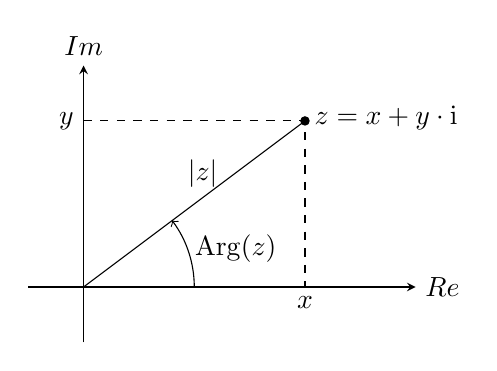
\begin{tikzpicture}[x=1em,y=1em]
%\pgfsetlinewidth{.5pt}
\draw[-stealth] (-2,0) -- (12,0) node[right] {$Re$}; 
\draw[-stealth] (0,-2) -- (0,8) node[above] {$Im$};
\draw (0,0) -- (8,6);
\draw[dashed] (0,6)--(8,6)--(8,0);
\draw (0,6) node[left] {$y$};
\draw (8,0) node[below] {$x$};
\draw (4.3,4.1) node {$|z|$};
\draw[fill] (8,6) circle (.15em);
\draw (8,6.1) node[right] {$z=x+y\cdot \mathrm{i}$};
\draw[->] (0,0) +(0:4) arc (0:37:4);
\draw (5.5,1.4) node {$\mathrm{Arg}(z)$};
\end{tikzpicture}\\[-3em]\rule{0pt}{0pt}
\end{center}
\caption{Representación gráfica de los números complejos}\label{repr-comp}
\end{figure}

%\newpage

\begin{definicion}%\label{def:funccomp}
En los siguientes apartados, $x,y\in\mathbb{R}$, $z\in\mathbb{C}$:
\begin{itemize}\setlength{\itemsep}{0pt}
\item
Módulo de un número complejo:
\[
|\cdot|\colon\mathbb{C}\to\mathbb{R}^+,\qquad |x+\mathrm{i} y| = \sqrt{x^2+y^2}; \quad |z|=\sqrt{z \bar{z}}
\]
\item
Argumento principal de un número complejo:\quad  $\mathrm{Arg}\colon\mathbb{C}^\ast\to[0,2\pi)$.\newline
Si $x=0$, entonces
\[
\mathrm{Arg}(\mathrm{i} y)=\dfrac{\pi}{2}, \text{ si } y > 0,\quad 
\mathrm{Arg}(\mathrm{i} y)=\dfrac{3\pi}{2}, \text{ si } y < 0;
\]
si $y=0$, entonces 
\[
\mathrm{Arg}(x)=0, \text{ si } x > 0,\quad 
\mathrm{Arg}(x)=\pi, \text{ si } x < 0;
\]
en cualquier otro caso, $\mathrm{Arg}(x+\mathrm{i} y)=\theta$, en donde $\operatorname{tg}\theta= \dfrac{y}{x}$,
\begin{align*}
& \theta\in [0,\pi]  \text{ si } y\ge 0, \\
& \theta\in (\pi,2\pi) \text{ si } y< 0.
\end{align*}
\end{itemize}
\end{definicion}
%
Hemos hecho uso de la siguiente notación: $\mathbb{C}^\ast=\mathbb{C}\smallsetminus\{0\}$.
En general, el superíndice~$\ast$ sobre cualquier conjunto numérico, indica que excluimos al número $0$.

Obsérvese que, por su definición, el módulo de un número complejo es siempre positivo y su argumento principal es un ángulo entre $0$ y $2\pi$.

\begin{ejemplo-br}
\begin{itemize}
\item $\mathrm{Re}(3-2\mathrm{i})=3$ 
\item $\mathrm{Im}(-1+\mathrm{i})=1$
\item $|1-\mathrm{i}| = \sqrt{1+1}=\sqrt2$
\item $\mathrm{Arg}(-1+\mathrm{i}) = \dfrac{3\pi}4$. Los dos ángulos entre $0$ y $2\pi$ cuyas tangentes son $-1$ son  $\dfrac{3\pi}4$ y $\dfrac{7\pi}4$, pero dado que la parte imaginaria es positiva, el argumento principal es el primero de ellos.\fej
\end{itemize}
\end{ejemplo-br}
%
\begin{proposicion}\label{pr:conjugado}
El operador conjugado verifica las siguientes propiedades:% si $z,w\in\mathbb{C}$
\[
\overline{z+w}=\overline{z}+\overline{w},\qquad
\overline{z\cdot w}=\overline{z}\cdot \overline{w}.
\]
\end{proposicion}

La demostración de esta proposición es una simple comprobación que debería ser fácilmente desarrollada por el estudiante. La principal consecuencia de esta propiedad es la siguiente.

\begin{proposicion}
Si $P(x)$ es un polinomio con coeficientes en $\mathbb{R}$ y $z\in\mathbb{C}$ es una raíz de $P$, entonces $\overline z$ también es raíz de $P$.
\end{proposicion}

En el ejemplo~\ref{ej:factor} de la página~\pageref{ej:factor} hemos visto que las raíces del polinomio $P(x)=x^4+4$ son:
\[
1+\mathrm{i},\quad
-1+\mathrm{i},\quad
1-\mathrm{i},\quad
-1-\mathrm{i},
\]
y efectivamente observamos que se verifica la propiedad de la proposición anterior.
La demostración del resultado es bastante simple; supongamos que
\[
P(x)=a_nx^n+\cdots+a_1x+a_0,
\]
y que $z\in\mathbb{C}$ es raíz de $P$; en el desarrollo siguiente, solo utilizamos la proposición anterior y que el conjugado de un número real es él mismo:
%
\begin{align*}
a_nz^n+\cdots+a_1z+a_0 & = 0 \\
\overline{a_nz^n+\cdots+a_1z+a_0} & = 0 \\
\overline{a_n}\cdot\overline{z}^n+\cdots+\overline{a_1}\cdot\overline{z}+\overline{a_0} & = 0 \\
{a_n}\overline{z}^n+\cdots+{a_1}\overline{z}+a_0 & = 0
\end{align*}
Por lo tanto, efectivamente $\overline z$ también es raíz del polinomio.
%
%\begin{ejemplo}\label{ej:eccomp}
%Vamos a resolver la ecuación
%\[
%z\bar{z}+3(z-\bar{z})=13+12\mathrm{i}
%\]
%En esta ecuación aparece la función conjugado y, por lo tanto, no son suficientes las propiedades algebraicas, así que necesitamos un tratamiento específico.
%Podemos utilizar dos métodos:
%\begin{enumerate}
%\item
%Si sustituimos $z$ por $x+\mathrm{i} y$, convertimos la ecuación en un sistema de ecuaciones reales cuyas soluciones son la parte real y la parte imaginaria de las soluciones de la ecuación inicial.
%Este es el método que hemos seguido en la ecuación $x^2-\mathrm{i}=0$ del ejemplo~\ref{ej:factor} (página~\pageref{ej:factor}).
%\item
%Aplicando el operador conjugado a la ecuación inicial, obtenemos una segunda ecuación; podemos considerar las dos ecuaciones como un sistema de ecuaciones en $\mathbb{C}$, de cuyas soluciones extraemos la solución de la ecuación inicial.
%\end{enumerate}
%Vamos a aplicar el segundo método a la ecuación propuesta para aclarar su funcionamiento.
%Si aplicamos el operador conjugado a los dos lados de la igualdad y aplicamos
%las propiedades de la proposición~\ref{pr:conjugado} obtenemos:
%\[
%\bar{z}z+3(\bar{z}-z)=13-12\mathrm{i}
%\]
%Si sustituimos $\bar z$ por $w$ en ambas ecuaciones, obtenemos el siguiente sistema en~$z$ y~$w$:
%\begin{align*}
%zw+3(z-w)&=13+12\mathrm{i} \\
%wz+3(w-z)&=13-12\mathrm{i}
%\end{align*}
%%
%Para resolverlo, basta con sumar y restar las dos ecuaciones, lo que nos lleva a un sistema equivalente pero más sencillo:
%\begin{align*}
%6z-6w &= 24\mathrm{i} \text{\quad(diferencia)}\\
%2zw &=26 \text{\quad(suma)}
%\end{align*}
%De la primera ecuación, deducimos que $w=z-4\mathrm{i}$, por lo que la segunda ecuación se convierte en
%\[
%z^2 - 4\mathrm{i} z-13=0,
%\]
%cuyas soluciones son $z=\dfrac{4\mathrm{i}\pm\sqrt{-16+52}}2=\pm3+2\mathrm{i}$.\fej
%\end{ejemplo}

%:2017 arg(zw)=arg(z)+arg(w)
%\begin{proposicion}\label{pr:argumento}
%El operador argumento verifica la siguiente propiedad:
%\[
%\mathrm{Arg}(zw)=\mathrm{Arg}(z)+\mathrm{Arg}(w)-2k\pi
%\]
%para algún $k\in\mathbb{N}$
%\end{proposicion}


\paragraph{Exponencial compleja y fórmula de De Moivre}

%Recordamos en esta sección las propiedades de las potencias y  logaritmos de números reales. 
%%
%\begin{proposicion-br}
%\begin{enumerate}
%\item $a^{x+y} = a^xa^y$
%\item $a^{xy} = (a^x)^y$
%\item $a^{-x} = 1/a^x$
%\item Si $a>1$ y $x<y$, entonces $a^x < a^y$.
%\item Si $0<a<1$ y $x<y$, entonces $a^x > a^y$.
%\item Si $0<a<b$ y $x>0$, entonces $a^x < b^x$
%\item Si $0<a<b$ y $x<0$, entonces $a^x > b^x$
%\end{enumerate}
%\end{proposicion-br}

Una representación alternativa para los números complejos se obtiene al usar la función exponencial.
Para introducirla, necesitamos en primer lugar, extender la definición de esta función a todos los números complejos.
%
\begin{definicion}
Definimos la función exponencial en el cuerpo de los números complejos como:\quad
$\mathrm{e}^{x+\mathrm{i} y} = \mathrm{e}^x(\cos y + \mathrm{i} \operatorname{sen} y)$.
\end{definicion}
%
Es evidente que esta definición es coherente con la exponencial sobre números reales, ya que si $y=0$:
\[
\mathrm{e}^{x+\mathrm{i} y}=\mathrm{e}^x(\cos y + \mathrm{i} \operatorname{sen} y) = \mathrm{e}^x(\cos 0 + \mathrm{i} \operatorname{sen} 0) = \mathrm{e}^x
\]
La otra razón por la que esta función se denomina exponencial es que comparte las propiedades algebraicas de su versión real.
%
\begin{proposicion-br}\label{pr:exp}
\begin{enumerate}
\item
$\mathrm{e}^z\ \mathrm{e}^w = \mathrm{e}^{z+w}$, para todo $z,w\in\mathbb{C}$
\item
$(\mathrm{e}^z)^n = \mathrm{e}^{nz}$, para todo $z\in\mathbb{C}$ y todo $n\in\mathbb{N}$
\end{enumerate}
\end{proposicion-br}
%
La segunda propiedad es una consecuencia de la primera y la demostración de la primera hace uso, solamente, de las fórmulas del seno y coseno de la suma de ángulos.
Consideramos $z=x_1+\mathrm{i} y_1$, $w=x_2+ \mathrm{i} y_2$, 
\begin{align*}
\mathrm{e}^z\ \mathrm{e}^w  &=\mathrm{e}^{x_1}\mathrm{e}^{x_2} (\cos y_1 + \mathrm{i}\operatorname{sen} y_1)(\cos y_2 + \mathrm{i}\operatorname{sen} y_2)\\
 &=\mathrm{e}^{x_1+x_2} (\cos y_1\cos y_2 - \operatorname{sen} y_1\operatorname{sen} y_2\\
&\ \qquad + \mathrm{i}(\operatorname{sen} y_1 \cos y_2 + \cos y_1
\operatorname{sen} y_2))\\
 &= \mathrm{e}^{x_1+x_2} (\cos( y_1 +  y_2) + \mathrm{i} \operatorname{sen}( y_1 +  y_2))\\
 & = \mathrm{e}^{x_1+x_2} \mathrm{e}^{\mathrm{i}( y_1+ y_2)} = \mathrm{e}^{z+w}
\end{align*}

\paragraph{Forma exponencial.}
Si $r=|z|$ y $\theta=\mathrm{Arg}(z)$, entonces 
\[
r\mathrm{e}^{\mathrm{i}\theta}=
r(\cos \theta + \mathrm{i} \operatorname{sen} \theta)=
r\cos \theta + \mathrm{i}\; r \operatorname{sen} \theta = z
\]
Por esta razón, la expresión $r\mathrm{e}^{\mathrm{i}\theta}$ se denomina \emph{forma exponencial} del número $z$.
Una representación alternativa a partir del módulo y argumento de un número complejo es la \emph{forma polar}, que se suele escribir como~$r_\theta$;
las dos representaciones son equivalentes en cuanto a sus consecuencias prácticas, pero preferimos utilizar la forma exponencial, ya que la manipulación de la misma se basa en las propiedades conocidas de la función exponencial.
%
\begin{ejemplo-br}
\begin{itemize}
\item
$-1 = \mathrm{e}^{\mathrm{i} \pi}$, ya que $|-1|=1$ y $\mathrm{Arg}(-1)=\pi$
\item
$-i = \mathrm{e}^{\mathrm{i}3\pi/2}$, ya que $|-i|=1$ y $\mathrm{Arg}(-i)=3\pi/2$
\item
$1-i =\sqrt2\mathrm{e}^{\mathrm{i}7\pi/4}$\fej
\end{itemize}
\end{ejemplo-br}

La igualdad $\mathrm{e}^{\mathrm{i}\theta} = \cos \theta + \mathrm{i} \operatorname{sen} \theta$, se conoce como \emph{igualdad de Euler} y en el caso particular $\theta=\pi$ conduce a una identidad que relaciona las constantes matemáticas más importantes:
\[
\mathrm{e}^{\mathrm{i}\pi}+1=0
\]

Por las propiedades de las potencias, obtenemos que
$(\mathrm{e}^{\mathrm{i}\theta})^n = \mathrm{e}^{\mathrm{i} n\theta}$ y a partir de aquí, deducimos la fórmula de De Moivre.
%
\begin{corolario}[Fórmula de De Moivre]
Para todo número natural $n$ y todo real $\theta$:
\[
(\cos\theta + \mathrm{i}\operatorname{sen}\theta)^n = \cos n \theta + \mathrm{i}\operatorname{sen} n \theta.
\]
\end{corolario}
%
Una importante aplicación de esta fórmula es obtener expresiones para simplificar funciones trigonométricas, según mostramos en los siguientes ejemplos.
%
\begin{ejemplo}
Si expandimos la igualdad de De Moivre para $n=2$ obtenemos:
\[
\cos 2 \theta + \mathrm{i}\operatorname{sen} 2 \theta=(\cos\theta + \mathrm{i}\operatorname{sen}\theta)^2
= \cos^2\theta + 2\mathrm{i}\operatorname{sen}\theta\cos\theta-\operatorname{sen}^2\theta 
\]
Igualando las partes reales y las partes imaginarias de ambos miembros, obtenemos la siguientes igualdades:
\begin{align*}
\cos 2 \theta &= \cos^2\theta -\operatorname{sen}^2\theta\\
\operatorname{sen} 2 \theta &= 2\operatorname{sen}\theta\cos\theta
\end{align*}
Es decir, hemos obtenido expresiones para escribir el seno y el coseno del doble de un ángulo en terminos del seno y el coseno del mismo ángulo.\fej
\end{ejemplo}

En combinación con el binomio de Newton, podemos obtener fórmulas similares para cualquier múltiplo, que nos ayudarán a simplificar expresiones en las que aparezcan distintos múltiplos de un mismo ángulo.

\begin{ejemplo}
Si expandimos la igualdad de De Moivre para $n=3$ obtenemos:
\begin{multline*}
\cos 3 \theta + \mathrm{i}\operatorname{sen} 3 \theta=(\cos\theta + \mathrm{i}\operatorname{sen}\theta)^3
=\\= \binom30\cos^3\theta + \binom31\mathrm{i}\cos^2\theta\operatorname{sen}\theta
+\binom32\mathrm{i}^2\cos\theta\operatorname{sen}^2\theta +\binom33\mathrm{i}^3\operatorname{sen}^3\theta=\\
= \cos^3\theta + 3\mathrm{i}\cos^2\theta\operatorname{sen}\theta
-3\cos\theta\operatorname{sen}^2\theta -\mathrm{i}\operatorname{sen}^3\theta
\end{multline*}
Igualando las partes reales y las partes imaginarias de ambos miembros, obtenemos la siguientes igualdades:
\begin{align*}
\cos 3 \theta &= \cos^3\theta -3\cos\theta\operatorname{sen}^2\theta \\
\operatorname{sen} 3 \theta &= 3\cos^2\theta\operatorname{sen}\theta-\operatorname{sen}^3\theta\fejeq
\end{align*}
\end{ejemplo}

En otras ocasiones, nos interesará un proceso opuesto al del ejemplo anterior, es decir, reducir potencias de funciones trigonométricas a expresiones en términos del seno y coseno de múltiplos del ángulo.
Para deducir estas expresiones partimos de las igualdades
%
\begin{align}
\cos x =\dfrac{\mathrm{e}^{\mathrm{i} x}+\mathrm{e}^{-\mathrm{i} x}}{2}\notag\\
\operatorname{sen} x =\dfrac{\mathrm{e}^{\mathrm{i} x}-\mathrm{e}^{-\mathrm{i} x}}{2\mathrm{i}}\label{def:sincos}
\end{align}
%
que se deducen fácilmente sumando y restando respectivamente, las siguientes:
%
\begin{align*}
\mathrm{e}^{\mathrm{i} x} & =\cos x + \mathrm{i} \operatorname{sen} x\\
\mathrm{e}^{-\mathrm{i} x} &=\cos x - \mathrm{i} \operatorname{sen} x
\end{align*}
%
Vemos a continuación un ejemplo de como usar la definición compleja de las funciones trigonométricas para el objetivo buscado.
%
\begin{ejemplo}
Vamos a transformar $\operatorname{sen}^2\theta$ en una expresión sin potencias:
\begin{align*}
\operatorname{sen}^2\theta  & = \left(\dfrac{\mathrm{e}^{\mathrm{i}\theta}-\mathrm{e}^{-\mathrm{i}\theta}}{2\mathrm{i}}\right)^2= \\
& = \dfrac{-1}4(\mathrm{e}^{2\mathrm{i}\theta}-2\mathrm{e}^{\mathrm{i}\theta}\mathrm{e}^{-\mathrm{i}\theta}+\mathrm{e}^{-2\mathrm{i}\theta})= \\
& = \dfrac{-1}4(\mathrm{e}^{2\mathrm{i}\theta}-2+\mathrm{e}^{-2\mathrm{i}\theta})= \\
& = \dfrac{-1}4((\mathrm{e}^{2\mathrm{i}\theta}+\mathrm{e}^{-2\mathrm{i}\theta})-2)= \\
& = \dfrac{-1}4(2\cos(2\theta)-2) = \dfrac{1-\cos 2\theta}2\fejeq
\end{align*}
\end{ejemplo}
%
En combinación con el binomio de Newton, podemos obtener fórmulas similares para cualquier potencia.
\begin{ejemplo}
Vamos a transformar $\operatorname{sen}^3\theta$ en una expresión sin potencias:
\begin{align*}
\operatorname{sen}^3\theta  & = \left(\dfrac{\mathrm{e}^{\mathrm{i}\theta}-\mathrm{e}^{-\mathrm{i}\theta}}{2\mathrm{i}}\right)^3 =\\
& = \dfrac{-1}{8\mathrm{i}}(\mathrm{e}^{3\mathrm{i}\theta}-3\mathrm{e}^{2\mathrm{i}\theta}\mathrm{e}^{-\mathrm{i}\theta}+3\mathrm{e}^{\mathrm{i}\theta}\mathrm{e}^{-2\mathrm{i}\theta}-\mathrm{e}^{-3\mathrm{i}\theta}) =\\
& = \dfrac{-1}{8\mathrm{i}}(\mathrm{e}^{3\mathrm{i}\theta}-3\mathrm{e}^{\mathrm{i}\theta}+3\mathrm{e}^{-\mathrm{i}\theta}-\mathrm{e}^{-3\mathrm{i}\theta})=\\
& = \dfrac{-1}{8\mathrm{i}}\big(\mathrm{e}^{3\mathrm{i}\theta}-\mathrm{e}^{-3\mathrm{i}\theta}-3(\mathrm{e}^{\mathrm{i}\theta}-\mathrm{e}^{-\mathrm{i}\theta})\big)=\\
& = \dfrac{-1}{8\mathrm{i}} (2\mathrm{i}\operatorname{sen}3\theta-3\cdot2\mathrm{i}\operatorname{sen}\theta)=\\
& = \dfrac{-1}{4} (\operatorname{sen}3\theta-3\operatorname{sen}\theta)\fejeq
\end{align*}
\end{ejemplo}
%
%Vamos a expresar $\cos 5\theta$ como polinomio en $\cos\theta$.
%\begin{align*}
%\cos 5 \theta & = \mathrm{Re}((\cos\theta+ \mathrm{i}\operatorname{sen} \theta)^5)\\
%&= \cos^5\theta +\binom52 (\cos^3\theta) \mathrm{i}^2(\operatorname{sen}^2 \theta)
%+\binom54 (\cos\theta) \mathrm{i}^4 (\operatorname{sen}^4 \theta) \\
%&= \cos^5\theta -10 \cos^3\theta\operatorname{sen}^2 \theta
%+5 \cos\theta\operatorname{sen}^4 \theta \\
%&= \cos^5\theta -10 \cos^3\theta(1-\cos^2 \theta)
%+5 \cos\theta(1-\cos^2 \theta)^2 \\
%&= \cos^5\theta -10 \cos^3\theta +10\cos^5 \theta
%+5 \cos\theta(1-2\cos^2 \theta+\cos^4\theta) \\
%&= 16\cos^5\theta -20 \cos^3\theta + 5\cos \theta
%\end{align*}
%
\begin{ejemplo}
%
Otra de las aplicaciones de la fórmula de De Moivre es el cálculo de las raíces de los números complejos, que nos aparecen en la resolución de ecuaciones polinómicas.
Por ejemplo, supongamos que queremos calcular los números complejos $w$, tales que $w^4=-4$; es decir, las \emph{raíces cuartas} de $-4$ y raíces del polinomio $P(z)=z^4+4$.
Para calcularlas, partimos de la forma exponencial de $-4$,
\[
-4 = 4\cdot\mathrm{e}^{\pi\mathrm{i}},\quad k\in\mathbb{Z}.
\]
Sin embargo, el ángulo $\pi$ no es el único que permite obtener una igualdad similar a la anterior; en general tenemos que:
\[
-4 = 4\cdot \mathrm{e}^{\mathrm{i}(\pi+2k\pi)}
\]
Las raíces $w=r\mathrm{e}^{\theta\mathrm{i}}$ que buscamos verifican entonces que:
\[
w^4= r^4 \mathrm{e}^{4\mathrm{i}\theta} = -4 = 4\cdot \mathrm{e}^{\mathrm{i}(\pi+2k\pi)}.
\]
De donde deducimos que
\[
r=\sqrt2\qquad \qquad
4\mathrm{i}\theta=\mathrm{i}(\pi+2k\pi)
\]
De la segunda igualdad, deducimos que solo cuatro valores de $\theta$ son argumentos principales de números complejos, los correspondientes a $k=0,1,2,3$:
\[
\theta_0=\frac{\pi}4,\quad
\theta_1=\frac{3\pi}4,\quad
\theta_2=\frac{5\pi}4,\quad
\theta_3=\frac{7\pi}4
\]
En consecuencia, $-4$ tiene cuatro raíces cuartas, cuyas representaciones gráficas en el plano complejo se pueden ver en la figura~\ref{fig:raices4-1}.
\begin{align*}
w_0&=\sqrt2 \mathrm{e}^{\mathrm{i}\theta_0}=\sqrt2 \mathrm{e}^{ \mathrm{i}\pi/4}
=\sqrt2\left(\frac1{\sqrt2}+\mathrm{i}\frac1{\sqrt2}\right)
= 1+\mathrm{i} \\
w_1&=\sqrt2 \mathrm{e}^{\mathrm{i}\theta_1}=\sqrt2 \mathrm{e}^{3\mathrm{i}\pi/4}
=\sqrt2\left(\frac{-1}{\sqrt2}+\mathrm{i}\frac1{\sqrt2}\right)
= -1+\mathrm{i}\\
w_2&=\sqrt2 \mathrm{e}^{\mathrm{i}\theta_2}=\sqrt2 \mathrm{e}^{5\mathrm{i}\pi/4}
=\sqrt2\left(\frac{-1}{\sqrt2}-\mathrm{i}\frac1{\sqrt2}\right)
= -1-\mathrm{i}\\
w_3&=\sqrt2 \mathrm{e}^{\mathrm{i}\theta_3}=\sqrt2 \mathrm{e}^{7\mathrm{i}\pi/4}
=\sqrt2\left(\frac1{\sqrt2}-\mathrm{i}\frac1{\sqrt2}\right)
= 1-\mathrm{i}
\end{align*}

\begin{figure}[htb]
\begin{center}
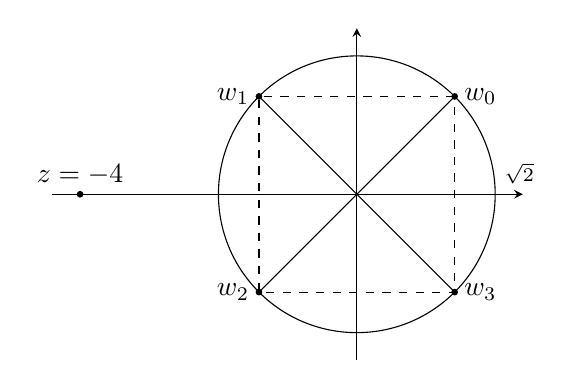
\begin{tikzpicture}[x=5em,y=5em]
\draw[-stealth] (-2.2,0) -- (1.2,0);% node[right] {$X$}; 
\draw[-stealth] (0,-1.2) -- (0,1.2);% node[right] {$Y$};
\draw (0,0) -- (.7071067811865475,.7071067811865475) node[right] {$w_0$};
\draw (0,0) -- (-.7071067811865475,.7071067811865475) node[left] {$w_1$};
\draw (0,0) -- (-.7071067811865475,-.7071067811865475) node[left] {$w_2$};
\draw (0,0) -- (.7071067811865475,-.7071067811865475) node[right] {$w_3$};
\draw (0,0) circle (1);
%\draw[dashed] (0,0) -- (1.732050807568877,1);
%
\draw[dashed] (.7071067811865475,.7071067811865475)  -- (-.7071067811865475,.7071067811865475) 
-- (-.7071067811865475,-.7071067811865475) 
-- (.7071067811865475,-.7071067811865475) --
(.7071067811865475,.7071067811865475);
%
\draw[fill] (.7071067811865475,.7071067811865475) circle (.1em);
\draw[fill] (-.7071067811865475,.7071067811865475) circle (.1em);
\draw[fill] (-.7071067811865475,-.7071067811865475) circle (.1em);
\draw[fill] (.7071067811865475,-.7071067811865475) circle (.1em);
\draw[fill] (-2,0) circle (.1em);
\draw (1.35,.15) node[left] {\scriptsize $\sqrt2$};
\draw (-2,0) node[above] {$z=-4$};
%
\end{tikzpicture}
\end{center}
\vspace{-2em}
\caption{Raíces cuartas de $z=-4$}\label{fig:raices4-1}
\end{figure}

Con estas raíces podemos factorizar el polinomio $P(z)$, tanto en $\mathbb{C}$ como en $\mathbb{R}$, de la siguiente manera:
\begin{eqnarray*}
P(z) &=& (z-1-\mathrm{i})(z-1+\mathrm{i})(z+1-\mathrm{i})(z+1+\mathrm{i})  \longrightarrow\mbox{factorización en $\mathbb{C}$}
\\ 
&=& (z^2-2z+2)(z^2+2z+1)  \hfill\longrightarrow\mbox{factorización en $\mathbb{R}$}
\end{eqnarray*}
Obsérvese que en el ejemplo~\ref{ej:factorPol4} (página~\pageref{ej:factorPol4}), resolvimos el mismo problema a partir de la ecuación polinómica. Debemos acostumbrarnos a que un mismo problema puede resolverse de varias formas y debemos aprender a elegir la forma más adecuada según los datos concretos.\fej
\end{ejemplo}
%
\begin{teorema}
Para cada número complejo $z=r\mathrm{e}^{i\theta}$ existen $n$ números complejos distintos $w_0,\dots,w_{n-1}$ que verifican $w_k^n=z$.
Estos números complejos son:
\[
w_k=\sqrt[n]{r}\exp\Big(\frac{\theta+2k\pi}{n} \mathrm{i} \Big),\qquad k=0,1,2,\dots,n-1
\]
\end{teorema}
Hemos utilizado en este enunciado una notación alternativa para la función exponencial
\[
\exp(x)=\mathrm{e}^x,
\]
que es de gran ayuda cuando escribimos expresiones grandes en el exponente.

\newpage

%\thispagestyle{empty}
%
%\ 
%
%\vfill
%\begin{center}
%(Esta página se ha dejado intencionalmente en blanco)
%\end{center}
%\newpage

\section*{Relación de ejercicios \thechapter.1}

\pagestyle{relaciones}

\begin{enumerate}

\item
Consideremos la definición de las funciones hiperbólicas que se presentan en la sección \ref{FuncHiperb} de la página \pageref{FuncHiperb} de los apuntes.
\begin{enumerate}
\item
Compruebe que $\cosh(0)=1$ y que $\operatorname{senh}(0)=0$ 
\item
Demuestre que $\dfrac{d}{dx}\cosh(x)=\operatorname{senh}(x)$, y que $\dfrac{d}{dx}\operatorname{senh}(x)=\cosh(x)$
%\item
%\item 
%En cada uno de los apartados anteriores, identifique las similitudes y las diferencias de las funciones hiperbólicas con respecto a las funciones trigonométricas. 
%\item
%Represente gráficamente las funciones $\cosh(x)$ y $\operatorname{senh}(x)$.
% (Para ello, determine los puntos de cortes con los ejes, intervalos de crecimiento y decrecimiento, concavidad y convexidad,\dots)
\end{enumerate}



\item 
Identidad hiperbólica fundamental.
\begin{enumerate}
\item 
Demuestre que $\cosh^2(x)-\operatorname{senh}^2(x)=1$ para todo $x\in\mathbb{R}$.    
\item
Utilice la fórmula del apartado anterior para obtener una expresión simplificada de la función $f(x)=\dfrac{x}{\sqrt{9+x^2}}$ cuando aplicamos el cambio de variable $x=3\operatorname{senh}(t)$
\end{enumerate}



\item Determine las soluciones de las siguientes ecuaciones:
\setcontadoralph
\begin{centrar}
\nitem
\(
(x-2)(x+2)=5
\)
\hfill
\nitem
\(
(x^3-2)\mbox{e}^{x^2-1}=0
\)
\end{centrar}
\begin{centrar}
\nitem
\(
(2x^2+3x-5)\ln(x^2-3)=0
\)
\hfill
\nitem
\(
3-2x = \sqrt{2x+3}
\)
\end{centrar}


\item Determine las soluciones de los siguientes sistemas de ecuaciones:
\setcontadoralph
\begin{centrar}
\nitem
\(\left\lbrace\begin{array}{rcc}
3x^2-3y &=& 0 \\
3y^2-3x &=& 0
\end{array}\right.\)
\hfill
\nitem
\(\left\lbrace\begin{array}{l}
x^2+y^2=1 \\
4-x^2=0
\end{array}\right.\) 
\hfill
\nitem
\(\left\lbrace\begin{array}{l}
x^2y+xy^2 = 0 \\
x^2-y^2=0
\end{array}\right.\)
\end{centrar}
\begin{centrar}
\nitem
\(\left\lbrace\begin{array}{rcc}
6x-2\lambda x &=& 0 \\
3y^2-2\lambda y &=& 0 \\
x^2+y^2 & = & 9
\end{array}\right.\)
\hfill
\nitem
\(\left\lbrace\begin{array}{rcc}
-\frac14 y\mbox{e}^{-\frac{xy}4}-2\lambda x &=& 0 \\
-\frac14 x\mbox{e}^{-\frac{xy}4}-2\lambda y &=& 0 \\
x^2+y^2 & = & 1
\end{array}\right.\)
\end{centrar}


\item
Desarrolle y simplifique las siguientes expresiones
\setcontadoralph
\begin{centrar}
\nitem
$\Big(4x-\dfrac12\Big)^4$ \hfill
\hfill
\nitem
$(x+y)^2-(x-y)^2$\hfill
\hfill
\nitem
$(x+y)^8-(x-y)^8$
\end{centrar}



\item
Ayudándose de la fórmula del binomio de Newton calcule: 
\[
\lm[n]{+\infty}\dfrac{(n+1)^5}{(n+1)^6-n^6}
\]


\item
Transforme los polinomios usando la técnica de completar cuadrados:
\setcontadoralph
\begin{centrar}
\nitem
$9x^2-6x+2$ \hfill
\hfill
\nitem
$5x^2+7x+2$\hfill
\hfill
\nitem
$3x^2+1$
\end{centrar}


\end{enumerate}



\newpage



\thispagestyle{empty}

\ 

\vfill
%\begin{center}
%(Esta página se ha dejado intencionalmente en blanco)
%\end{center}
\newpage

\section*{Relación de ejercicios \thechapter.2}

\pagestyle{relaciones}

\begin{enumerate}

\item
Determine la forma binómica de los siguientes números complejos.
\setcontadoralph
\begin{centrar}
\nitem
$(5 + 3\mathrm{i})(2-\mathrm{i})-(3+\mathrm{i})$
\hfill
\nitem
$\dfrac1{\mathrm{i}}$
\hfill
\nitem
$\dfrac{18+\mathrm{i}}{3-4\mathrm{i}}$
\hfill
\nitem
$\mathrm{i}^{-17}$
\hfill
\nitem
$(1-2\mathrm{i})^5$
\end{centrar}


\item
Resuelva en $\mathbb{C}$ la siguiente ecuación y exprese la solución en forma binómica:
\[
\dfrac{2z}{1+\mathrm{i}}-\dfrac{2z}{\mathrm{i}} = \dfrac{5}{2+\mathrm{i}}
\]


\item
Resuelva en $\mathbb{C}$ el siguiente sistema y exprese las soluciones en su forma binómica:
\[\left\{\begin{array}{ll}
4z+3w=23\\
z+\mathrm{i} w=6+8\mathrm{i}
\end{array}\right.\]

\item
Resuelva en $\mathbb{C}$ la siguiente ecuación y exprese la solución en forma binómica:
\[
z^2+2\overline{z}-1=0
\]


\item
Factorice en $\mathbb{R}$ y en $\mathbb{C}$ el polinomio $x^3-5x^2+11x-15$.
¿Cuáles son las soluciones de la ecuación $x^3-5x^2+11x-15=0$?

\item
Factorice en $\mathbb{R}$ y en $\mathbb{C}$ el polinomio $x^4-4$.
¿Cuáles son las soluciones de la ecuación $x^4-4=0$?

\item
Utilice el procedimiento que se describe en el ejemplo \ref{ej:factorPol4} para factorizar en $\mathbb{R}$ y en $\mathbb{C}$ el polinomio $x^4+9$ 

\item
Exprese en forma exponencial los siguientes números
\setcontadoralph
\begin{centrar}
%$1$,\hfill
%$-1$,\hfill
%$\mathrm{i}$,\hfill
%$-\mathrm{i}$,\hfill
% $-1-\mathrm{i}$.
%,\qquad(2-\mathrm{i})(2+\mathrm{i})
\nitem
$1-\mathrm{i}$\hfill
\nitem
$-\sqrt3+\mathrm{i}$\hfill
\nitem
$-1-\mathrm{i}\sqrt3$%,\hfill
%\nitem
%$(1+\mathrm{i})(-\sqrt3+\mathrm{i})$.
\end{centrar}


\item
Escriba $\operatorname{sen} 4\theta$ en términos de $\operatorname{sen}\theta$ y $\cos\theta$


\item
\begin{enumerate}
\item
Exprese $\operatorname{sen}^6\theta$ en función del seno y coseno de múltiplos de $\theta$
\item
Utilice la expresión obtenida en el apartado anterior y las \emph{propiedades de linealidad} de la integral para calcular la integral $\displaystyle\int\operatorname{sen}^6\theta\mathrm{d}\theta$
\end{enumerate}


\item Encuentre y represente gráficamente los siguientes números: las raíces quintas de~$-1$, 
las raíces sextas de~$-\mathrm{i}$, las raíces cuartas de $32(1-\mathrm{i}\sqrt{3})$.\newline
Describa la representación gráfica de las raíces $n$-ésimas de un número complejo.


\end{enumerate}


\newpage

\thispagestyle{empty}

\ 

\vfill
%\begin{center}
%(Esta página se ha dejado intencionalmente en blanco)
%\end{center}
\newpage


\section*{Relación de ejercicios \thechapter.3 - REPASO}

\begin{enumerate}

%%% EJERCICIOS DE RESOLUCIÓN DE SISTEMAS DE ECUACIONES NO LINEALES.

\item Determine las soluciones de los siguientes sistemas de ecuaciones:
\begin{enumerate}
\item
\(\left\lbrace\begin{array}{rcc}
8x^3+8x+8y &=& 0 \\
2y+8x+4 &=& 0
\end{array}\right.\)
\item
\(\left\lbrace\begin{array}{rcc}
2x\mbox{e}^{x-y}+(x^2+y^2)\mbox{e}^{x-y} &=& 0 \\
2y\mbox{e}^{x-y}-(x^2+y^2)\mbox{e}^{x-y} &=& 0
\end{array}\right.\)
\item
\(\left\lbrace\begin{array}{rcc}
3x^2-2\beta x &=& 0 \\
3y^2-2\beta y &=& 0 \\
x^2+y^2 & = & 1
\end{array}\right.\)
\end{enumerate}


%%% EJERCICIOS DE BINOMIO DE NEWTON

\item Use la fórmula del binomio de Newton para desarrollar las siguientes potencias:
\setcontadoralph
\begin{center}
\begin{tabular}{l@{\qquad\quad}l@{\qquad\quad}l}
\nitem $(a+b)^7$ &
\nitem $(x-1)^4$ &
\nitem $\left(2x^3-\dfrac{2}{5x^2}\right)^2$ \\[1em]
\nitem $(x-2)^5$ &
\nitem $(1-2x)^3$ &
\nitem $(z+1/2)^3$
\end{tabular}
\end{center}


%%% EJERCICIOS DE NÚMEROS COMPLEJOS

\item
Simplifique y exprese el resultado en forma binómica:
\setcontadoralph
\begin{centrar}
\nitem
$\dfrac{1-\mathrm{i}}{1+\mathrm{i}}$\hfill
\nitem
$\dfrac{5}{1-3\mathrm{i}} - \dfrac{5}{1+3\mathrm{i}}$\hfill
\nitem
$\frac12(1+\mathrm{i})^2$\hfill
\nitem
$\mathrm{i}^{2014}$\hfill
\nitem
$(1-\mathrm{i})^8$
\end{centrar}

\item
Exprese en forma binómica las soluciones de la siguiente ecuación:
\[
\dfrac{1}{z}=\dfrac{2}{2+3\mathrm{i}} + \dfrac{\mathrm{i}}{3-2\mathrm{i}}
\]




\item Resuelva el siguiente sistema de ecuaciones: $\left\{\begin{array}{ll}
z-w+u=2-\mathrm{i}\\
z+\mathrm{i} w=6+8\mathrm{i}\\
w+2\mathrm{i} u=-2\mathrm{i}
\end{array}\right.$

\item Resuelva la siguiente ecuación y exprese la solución en forma binómica:
% SIN escribir la incógnita en su forma binómica.
\[
z+\bar{z}\mathrm{i}-5=\dfrac{3-z\bar{z}}{2\mathrm{i}}
\]

\item
%Sin operar la expresión, 
Calcule el módulo de\quad $z=\dfrac{(1+2\mathrm{i})^3(4-3\mathrm{i})^4}{(3+4\mathrm{i})^4(2-\mathrm{i})^3}$

\item Exprese en forma exponencial los siguientes números
\setcontadoralph
\begin{centrar}
\nitem
$\sqrt2-\mathrm{i}\sqrt2$\hfill
\nitem
$\big(\sqrt2-\mathrm{i}\sqrt2\big)^2$\hfill
\nitem
$-2+2\mathrm{i}$\hfill
\nitem
$-\sqrt3-\mathrm{i}$\hfill
\nitem
$1-\mathrm{i}\sqrt3$
\end{centrar}


\item
Calcule las siguientes exponenciales complejas
\setcontadoralph
\begin{centrar}
\nitem
$\exp(1-\pi\mathrm{i})$\hfill
\nitem
$\exp\big(1-\frac{5\pi}{3} \mathrm{i}\big)$\hfill
\nitem
$\mbox{e}^{\frac{\pi}{2} \mathrm{i}} \mbox{e}^{1-\frac{3\pi}{4} \mathrm{i}}$
\end{centrar}

\item Exprese $\operatorname{sen} 3\theta$, $\cos 6\theta$ y $\operatorname{sen} 5\theta$ como polinomios en $\operatorname{sen}\theta$.

\item Exprese $\cos^4\theta$, $\operatorname{sen}^3\theta$ y $\cos^5\theta$ en términos de senos y cosenos de múltiplos de~$\theta$.

\item\label{ej:pi12}
Consideramos los números complejos $z=1+\mathrm{i}$, $w=-\sqrt3+\mathrm{i}$
\begin{enumerate}
\item
Calcule y simplifique el producto $zw$
\item
Utilizando la forma exponencial de $z$ y $w$, calcule el producto $zw$ y exprese el resultado en forma exponencial y forma binómica.
\item
A partir de los resultados obtenidos en los dos apartados anteriores, deduzca el valor de $\cos\frac{\pi}{12}$, $\operatorname{sen}\frac{\pi}{12}$ y $\operatorname{tg}\frac{\pi}{12}$
\end{enumerate}

\item
\begin{enumerate}
\item
Calcule las raíces cúbicas de $4\sqrt{2}+4\sqrt{2}\mathrm{i}$ y expréselas en forma binómica.\newline
(Indicación: use los valores de $\operatorname{sen}\frac{\pi}{12}$ y  $\cos\frac{\pi}{12}$ calculados en el ejercicio anterior.)

\item
Represente gráficamente las raíces calculadas en el apartado anterior.
\end{enumerate}

\item
Factorice en $\mathbb{R}$ y en $\mathbb{C}$ los siguientes polinomios.
% (utilice los métodos aprendidos a lo largo del tema y en la relación de ejercicios).
\setcontadoralph
\begin{center}
\begin{tabular}{l@{\qquad}l@{\qquad}l}
\nitem
$z^3+8$ &
\nitem
$y^4+81$ &
\nitem
$z^4+5z^2+4$\\[.5em]
\nitem
$t^6-2t^4+4t^2$ &
\nitem
$3x^3-x^2-7x+5$ &
\nitem
$x^3-12x+16$
\end{tabular}
\end{center}

\end{enumerate}

% Descomentar estas líneas si el capítulo acaba en página impar

%\newpage
%
%\thispagestyle{empty}
%
%\ 
%
%\vfill
%%\begin{center}
%%(Esta página se ha dejado intencionalmente en blanco)
%%\end{center}
%\newpage

\endinput
